\documentclass[11pt]{article}
%\usepackage[acronym,nonumberlist,toc]{glossaries}
\usepackage{graphicx}
\usepackage{times}
\usepackage{amsmath}
\usepackage[section]{placeins}
%\usepackage{subfigure}
\usepackage{subcaption}
\usepackage{booktabs}
\usepackage[version=4]{mhchem}
\usepackage{wrapfig}
\usepackage{textcomp}
\usepackage{geometry}
\geometry{left=2.5cm,right=2.5cm,top=2.5cm,bottom=2cm}
\usepackage{multirow}
\usepackage{color}
\usepackage[sort,numbers]{natbib}
\usepackage{authblk}



\title{Prediction of self-healing in engineered cementitious composite: Machine learning comparative analysis}
\author{Guangwei Chen $^{1,2,*}$, Patrick Tang $^{1}$, Shuo Chen $^{1}$, Shangyong Wang $^{1}$, and Hongzhi Cui $^3$}


\affil[1]{The University of Newcastle,  Callaghan, 2308, NSW, Australia}
\affil[2]{Qiannan Normal College of Nationalities, Guizhou, China}
\affil[3]{College of Civil and Transportation Engineering, Shenzhen University, Shenzhen 518060, China}
\date{}  

\begin{document}


%
%\address{%
%	$^{1}$ \quad The University of Newcastle,  Callaghan, 2308, NSW, Australia  }
%
%
%\corres{Correspondence: guangwei.chen@uon.edu.au}
%
%
%% Abstract (Do not insert blank lines, i.e. \\) 
%\abstract{Engineered cementitious composite (ECC) is a unique material which can significantly contribute to self-heal cracks based on ongoing hydration \cite{yildirim2014influence}. As model-free approaches eliminating the need of new models for different prediction problems, machine learning algorithms have been widely used to model the properties of concrete. This paper aims to provide a comparative analysis on the performance of machine learning models, the individual and ensemble methods, in predicting self-healing capability of ECC. These models include four individual methods (linear regression (LR), back-propagation neural network (BPNN), classification and regression tree (CRAT), and support vector regression(SVR)), three ensemble methods (bagging, AdaBoost, and stacking) with each of the four individual models used as the based learner. The results shows that the stacking model performs the best with the lowest error and highest accuracy on the self-healing capability prediction of ECC. On average, all ensemble models improve the prediction performance of the individual model which is used as the base learner in the ensemble model. }

% Keywords
%\keyword{ECC, self-healing, machine learning, ensemble method}
\maketitle

\begin{abstract}
	Engineered cementitious composite (ECC) is a unique material which can significantly contribute to self-heal cracks based on ongoing hydration. As model-free approaches eliminating the need of new models for different prediction problems, machine learning algorithms have been widely used to model the properties of concrete. This paper aims to provide a comparative analysis on the performance of machine learning models, the individual and ensemble methods, in predicting self-healing capability of ECC. These models include four individual methods (linear regression (LR), back-propagation neural network (BPNN), classification and regression tree (CRAT), and support vector regression(SVR)), three ensemble methods (bagging, AdaBoost, and stacking) with each of the four individual models used as the based learner. The results shows that the stacking model performs the best with the lowest error and highest accuracy on the self-healing capability prediction of ECC. On average, all ensemble models improve the prediction performance of the individual model which is used as the base learner in the ensemble model. 
\end{abstract}

\smallskip
\noindent \textbf{Keywords } ECC, self-healing, machine learning, ensemble method

	\section{Introduction}
	
	A market research project was commissioned by Materials for Life (M4L), which shows cracking damage in concrete was experienced more than any other problems \cite{gardner2018survey}. Moreover, cracks are primarily responsible for the reduction of the strength and stiffness of the concrete structure. Annual cost spent on maintenance, refurbishment and repair such cracks to prolong the service life of infrastructure is estimated around 50\% of the annual construction budget in European \cite{cailleux2009investigations}. Based on such circumstances, self-healing cementitious materials are proposed by M4L research team. They state self-healing cementitious materials benefit water retaining infrastructure to reduce repair costs over a premium in the capital material cost \cite{gardner2018survey}. 
	
	The inspiration of self-healing comes from biomimicry concept and the healing process in living nature \cite{ramadan2017modeling}. For example, the skin of humans or animals can biologically repair itself from scars injured area. According to the healing mechanism, self-healing can be  categorised into two major classes, autogenous healing and autonomous healing \cite{tang2015robust}. The former indicates the self-healing ability results from the physical and/or chemical composition of the cementitious matrix. And the latter states the self-healing mechanism is triggered by some biological agents, such as bacteria which are artificially presented in the cementitious matrix.
	
	Generally, autogenous self-healing in concrete is attributed to two major mechanisms including (1) further hydration of cement particles and/or swelling of calcium silicate hydrate; (2) calcium hydroxide carbonation \cite{edvardsen1999water}. Researchers have proposed the maximum crack widths as 10$\mu$m \cite{jacobsen1995sem}, 100 $\mu$m \cite{reinhardt2003permeability}, 200 $\mu$m \cite{csahmaran2008influence}, 205 $\mu$m \cite{edvardsen1999water} and 300 $\mu$m \cite{clear1985effects} are self-healed completely \cite{sahmaran2013self}. 
	
	Engineered cementitious composite (ECC), as an autogenous self-healing of concrete, is a high performance fiber-reinforced cementitious composite designed with micro-mechanical principles \cite{kamada2000effects}. It features high tensile ductility with a moderate fiber-volume fraction \cite{li1998innovations,ozbay2013self} - typically 2\% by volume which is designed to promote the self-healing ability \cite{tang2015robust}. 
	% for over 300 $\mu$m cracks
	
	The intrinsic self-healing ability of ECC is complex and uncertain due to material nature, interactivity between different composites in the cementitious matrix and its interaction with the exposed environment \cite{wu2012review}, and unpredictable crack location, orientation and width \cite{huang2013characterization}. Several studies explored the influence of different factors, such as limestone powders (LP) \cite{suleiman2019visualization,zhou2008developing}, fly ash (FA) \cite{li2007self,zhang2014investigating}, hydrate lime \cite{yildirim2014influence}, water/binder ratio \cite{yang2005self}, water permeation \cite{sahmaran2007transport} and different curing condition (air, carbon dioxide, wet/dry and water) \cite{qian2010influence} on self-healing behavior. However, the relationship between multiple factors is questionable and non-linear, which makes it difficult to predict self-healing mathematically based on available data. \textcolor{blue}{Moreover, mathematical models based on empirical data are generally in regression forms which cannot be used for problem containing independent variables, such as prediction of self-healing ability of ECC, because of less accuracy and more assumption in regression form (linear, non-linear, etc.) \cite{alshihri2009neural}.}
	
	%Moreover, it is expensive and time-consuming to quantify self-healing capability by conducting experiments only. 
	
	To compensate for the drawbacks of mathematical models with multiple interaction variables, machine learning algorithms are applied to many civil engineering problems. Many research works have been conducted using machine learning algorithms for the prediction of various properties of concrete. Gilan et al.\cite{gilan2012hybrid} established a hybrid Support Vector Regression (SVR) - Particle Swarm Optimization (PSO) algorithm model to predict the compressive strength and Rapid Chloride Penetration Test (RCPT) results of concretes containing metakaolin. Yan et al. \cite{yan2017evaluation} predicted bond strength of glass fiber-reinforced polymer bar concrete by Artificial Neural Network (ANN) with Genetic Algorithm (GA). Yaseen et al.\cite{yaseen2018predicting} proposed a machine learning method called Extreme Learning Machine (ELM) to predict the compressive strength of lightweight foamed concrete. 
	
	Compared with single method, several scholars compares the performance of various machine learning algorithms on predicting concrete properties to indicate the best modeling method. Yan and Shi \cite{yan2010prediction} reported that SVR is better than other individual methods to predict elastic modulus of normal and high strength concrete. Chou \cite{chou2014machine} compared performance of individual and ensemble methods for predicting the mechanical properties of high performance concrete. Reuter et al. \cite{reuter2018comparative} employed three individual approaches to model concrete failure surfaces.  Sobhani et al. \cite{sobhani2010prediction} indicates ANN and a proposed fuzzy inference system are more feasible than traditional regression models on predicting no-slump concrete. Omran et al. \cite{omran2016comparison} compared prediction results of environmentally friendly concrete compressive strength by using three individual methods, two ensemble methods, and four regression tree models.
	
	\textcolor{red}{red letters represent comments that will be delete later.}, \textcolor{blue}{blue letters represent new added materials.}
	
	Although researchers have been utilized different machine learning algorithms to anticipate and evaluate various properties of concrete, the application of machine learning focusing on self-healing is considerably rare. 
	
	\textcolor{blue}{
		Mauludin and Oucif \cite{mauludin2019modeling} reviewed the methods used for modeling autogenous self-healing in concrete, which mainly fell into two categories, numerical simulation and machine learning. And the only machine learning model reviewed in their study was proposed by Ramadan et al. \cite{ramadan2017modeling}. A GA-ANN model was applied in \cite{ramadan2017modeling} to predict the self-healing ability of cement-based materials using dataset collected from literatures, and stated that the proposed GA–ANN model was capable of capturing the complex effects of various self-healing agents (e.g., biochemical material, silica-based additive, expansive and crystalline components) on the self-healing performance in cement-based materials. However, they didn't compare their prediction performance with linear regression or neural network model to present the advantage of proposed GA-ANN model eliminating the data dependence of models.}  
		
		
		\textcolor{red}{Comments only shown in this draft: In \cite{ramadan2017modeling}, the prediction accuracy $R^2$ is over 99.7\%, which is doubtable, especially on training dataset. Generally, over 99.7\% prediction accuracy means the relationship between input variables and the output variable fit into a mathematical rule or expression. However, there is measurement errors in all engineering problems, and this measurement error is stochastic. That means we almost impossible to find out a mathematical model to present the relationship between input and output variables explicitly.}
	
	\textcolor{blue}{
	Wang et al. \cite{wang2019towards} used ANN and ensemble classification models to implement binary prediction (healed or not)	of self-healing materials based on 30 samples. However, the regression models were conducted by numerical simulations which assumed the relationship between the input and output variables following some logistic regression models. Later, \cite{chaitanya2020prediction} used an ANN model to predict the self-healing property, compressive strength, of Ground Granulated Blast Furnace slag using 51 samples collected from lab experiment. However, these two papers lacks prediction performance comparison on validation and testing dataset, and benchmark models, such as linear regression model. Moreover, limited number of samples (data) may not be enough for training a reliable model.}	 
		 
	A comparative study was conducted by \cite{zhuang2019prediction} using SVR, Decision Tree Regression (DTR), Gradient Boosting Regression (GBR), ANN, Bayesian Ridge Regression (BRR) and Kernel Ridge Regression (KRR) to predict the self-healing capability of bacteria-based concrete. \textcolor{blue}{The results showed GBR (with $R^2$ 0.736 on testing dataset and 0.93 on training dataset) was superior to other models (with $R^2$ less than 0.7 on both training and testing dataset on most models). In their study, extensive experiments with different combinations of influencing variables were implemented to generate empirical dataset. However, only three variables, the number of bacteria, the healing time and the initial crack width, were selected to predict the crack close percentage as the output.  }
	
	To the best of our knowledge, no studies have applied a ML model to predict the self-healing of ECC, let alone presenting a comparative analysis by comparing prediction performance of individual and ensemble ML models. Thus, the objective of this paper is to compare multiple machine learning techniques to identify the most reliable model for predicting the self-healing behavior of ECC, which is also considered as a baseline prediction model for other advanced models in our future works. 

	
	In this paper, four individual methods including linear regression (LR), SVR, back-propagation neural network (BPNN), and classification and regression tree (CART) were used to predict self-healing capability of ECC, which were then constructed as base learners in three ensemble methods naming bagging, AdaBoost and stacking for prediction. Variable controlled experiments were implemented to collect empirical data used in ML models, where only the input variables of ML models are variables in experiments, and other impact factors were controlled constantly in experiments. Empirical data collected from variable controlled experiments were preprocessed and then split by a 10-fold cross-validation algorithm (details refer to Section \ref{cross}) to avoid overfitting and minimize bias associated with various range of data. Figure \ref{fig:structure} summarizes the steps that were performed for predicting self-healing capability of ECC. 
	
	\begin{figure}	
		\begin{center}
			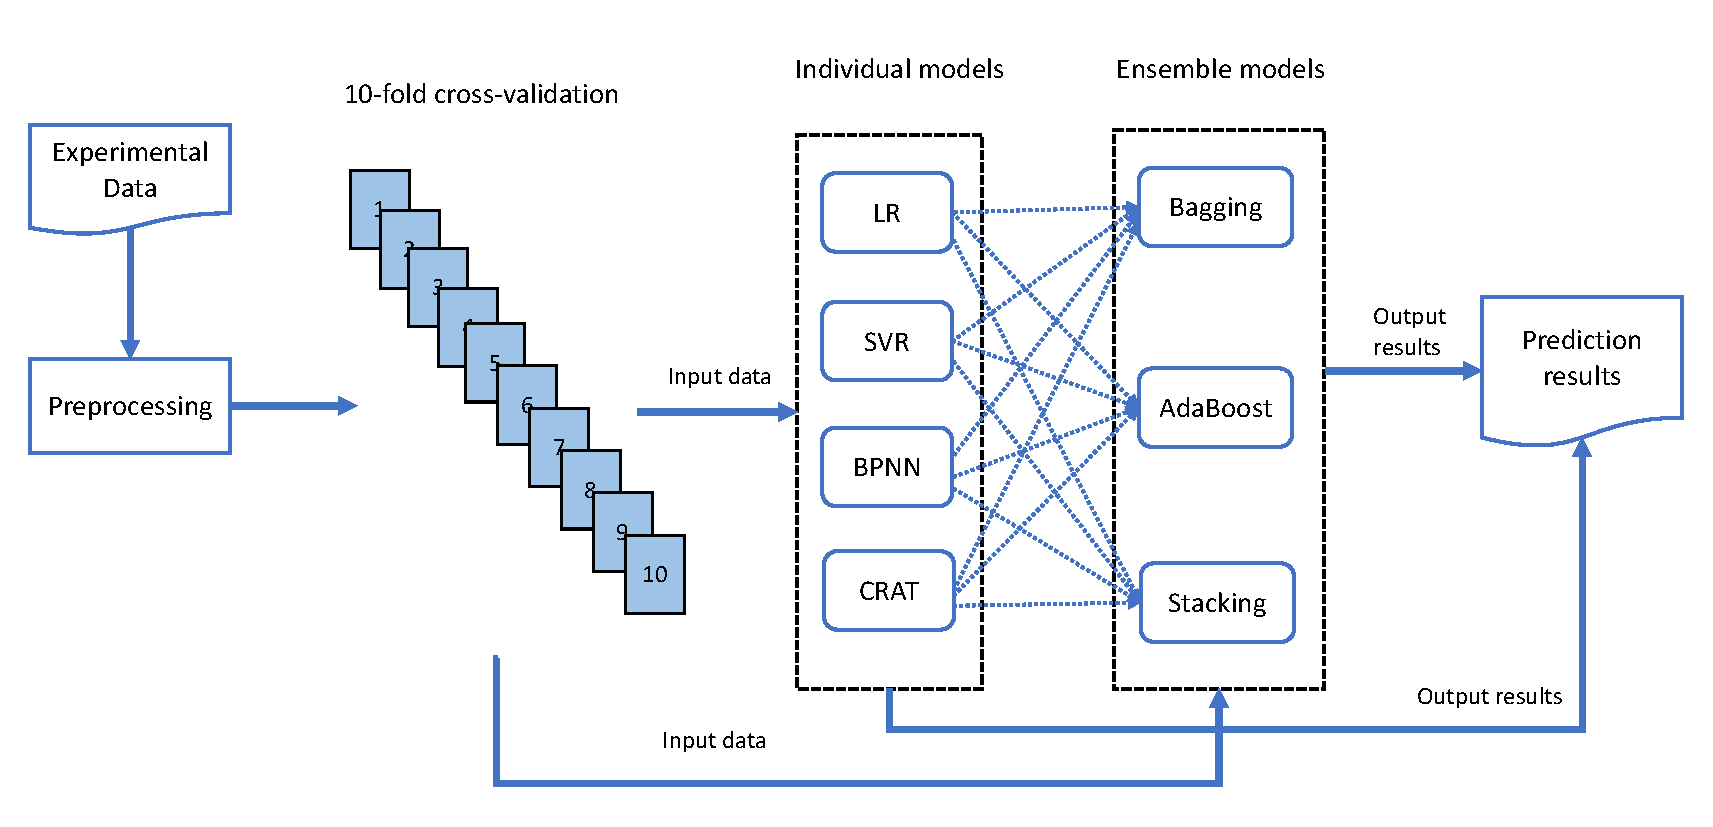
\includegraphics[width=\textwidth]{structure.pdf}
		\end{center}
		\caption{Flow chart of implementing prediction models for self-healing capability of ECC}
		\label{fig:structure}
	\end{figure}
	
	
	The reminder of this paper is organized as follows. Section \ref{lab} present the experimental program that devotes to materials used in preparing ECC mixtures and preprocessing of collected samples from experiments. It is followed by methodology Section \ref{meth} which describes the concepts and formulations of individual and ensemble models used for predicting self-healing capability of ECC. Validation and Evaluation methods are introduced in Section \ref{4}. After that, computational results of all individual and ensemble models are presented and compared in Section \ref{result}, which demonstrate the superiority of machine learning algorithms for prediction of the self-healing capability of ECC. Finally, Section \ref{con} draws some conclusions from this work and suggests directions for future research.
	
	% 
	%%%%%%%%%%%%%%%%%%%%%%%%%%%%%%%%%%%%%%%%%%
	
	\section{Experimental Program}
	\label{lab}
	
	\subsection{Materials and Mixture Proportion}
	

	
	
	In order to investigate the influence of mix composition on the self-healing capability of ECC, nine ECC mixes were prepared for experimental analysis. The binder composition of ECC mixes were general purpose cement (GPC), fly ash (FA), silica fume (SF), hydrated lime powder(LP), fine sand, polyvinyl alcohol fibers (PVA), as well as water and high range water reducing admixture (HRWR). GPC and FA were supplied by Boral in accordance with Australian Standard AS 3972-2010, while LP was the Adelaide Brighton Hydrated Lime with a specific gravity of 2.2-2.3, and a typical fineness of 0.1\% retained on a $75 \mu m$ sieve and less than 0.05\% on a $250 \mu m$ sieve. The physical and chemical properties of cementitious materials are shown in Table \ref{cm}. Fine sand was employed with an average grain size of 150 $\mu$m and fineness modulus of 2.01. PVA were produced by Domocrete and their mechanical and geometrical properties are described in Table \ref{pva}.
	
		\begin{table}[!h]
		\centering
		\caption{Physical and chemical properties of cementitious materials}
		\begin{tabular}{lcccc}
			\toprule
			\textit{Chemical composition} (\%) &	GPC &	FA&	LP&	SF\\
			\midrule
			Silica (\ce{SiO2})	&19.8 &	65.90 &	1.8&	95.10	\\
			Alumina (\ce{Al2O3})	& 5.3&	24.0&	0.5&	0.21	\\
			Iron oxide (\ce{Fe2O3}) &3.0	&2.87&	0.6	&0.29	\\
			Calcium oxide (\ce{CaO}) &	64.2 &	1.59 &	72.0 &	-	\\
			Magnesia (\ce{MgO})&1.3 &	0.42 &	1.0	 & -	\\
			\ce{R2O}	&0.6 &	1.93 &	- &	- \\
			Sulfur trioxide (\ce{SO3}) &	2.7	& - & - & -	\\
			Titanium oxide (\ce{TiO2})	&0.28 &	0.91 &	-  & -	\\
			Manganic oxide (\ce{Mn2O3}) & 0.22 & - & - & - \\	
			Zirconia (\ce{ZrO2}) + Hafnium (\ce{HfO2}) & -  & - & -	&3.46	\\
			& & & &\\
			Loss on ignition (\%) &	2.8	&1.53&	24.0&	1.4	\\
			Density ($g/cm^3$)	& 3.08 &	2.43 &	2.25 &	2.26	\\
			Specific surface area ($m^2/kg$) &	- &	655	&460 &	$1.5 \times 10^4$	\\
			\bottomrule
		\end{tabular}
		\label{cm}
	\end{table}
	
	\begin{table}[!h]
		\centering
		\caption{Properties of PVA}
		\begin{tabular}{ccccccc}
			\toprule
			Length &Length/&	Young’s modulus &	Elongation &Tensile strength &	Density \\
			(mm)	& diameter ratio & (MPa) & (\%)	 & (MPa) & (g/cm3) \\
			\midrule
			8&	200	&42000&	7&	1600&	1.3
			\\
			\bottomrule
		\end{tabular}
		\label{pva}
	\end{table}
	
	During the production process, a planetary-type mixer of 50 L capacity was used to produce specimens with water to cementitious materials (W/CM) ratio of 0.29, and sand to CM (PC + FA + LP+SF) ratio of 0.36. All the fine aggregates were in saturated surface dried condition prior to concrete mixing. Among nine ECC mixes, a mixture was prepared with GPC and FA while other mixtures were obtained by replacing part of the FA by SF or LP. For example, ECC mixture represented by FA70 stated that 70\% of the cementitious materials weight was FA, and by FA60-SF10 indicated that 10\% of the FA was replaced by SF. The details of mix proportion for all nine mixtures are shown in Table \ref{mx}. 
	
	
	\begin{table}[!tp]
		\centering
		\caption{Mix proportion of all ECC mixtures}
		\begin{tabular}{lccccccccc}
			\toprule
			Mix&	Water/CM	&Sand&	Water&	fibre (V)&	GPC	&Fly ash&	SF&	LP&	HRWR
			\\
			\midrule
			FA70&	0.29&	419.67&	338.07	&26	&349.73&	816.03	&0.00&	-	&5.13
			\\
			FA65-SF5&	0.29&	419.67&	338.07&	26	&349.73	&757.74&	58.29&	-&	5.13
			\\
			FA60-SF10	&0.29&	419.67&	338.07&26&	349.73&	699.45&	116.58	&-&	5.13
			\\
			FA55-SF15&	0.29&	419.67&	338.07&	26&	349.73&	641.16&	174.86	&-&	5.13
			\\
			FA65-LP5&	0.29&	419.67	&338.07&	26	&349.73	&757.74	&-	&58.29&	5.13
			\\
			FA60-LP10&	0.29&	419.67&	338.07&	26&	349.73	&699.45	&-	&116.58	&5.13
			\\
			FA55-LP15&	0.29&	419.67&	338.07&	26&	349.73	&641.16	-&	174.86	&5.13
			\\
			FA55-SF5-LP10&	0.29&	419.67&	338.07	&26&	349.73&	641.16	&58.29	&116.58	&5.13
			\\
			FA55-SF10-LP5	&0.29	&419.67	&338.07	&26	&349.73	&641.16	&116.58	&58.29	&5.13
			\\
			\bottomrule
		\end{tabular}
		\label{mx}
	\end{table}
	
	\subsection{Experiment}
	\label{experi}
	
	To prepare cement pastes, solid ingredients including cement, mineral admixtures and sand were first mixed for 30 seconds. Water pre-mixed with HRWR was then added into dry solid ingredients and mixed for 2 minutes. After that, PVA were slowly added into the matrix which were blended continually until PVA distributed evenly. For creating ECC composite cylinders, cement pastes were cast into standard moulds with dimension of $\O 100mm \times 200mm$ which were demolded after 24 hours. The demolded cylinders were cured in a curing room with a temperature of $23 \pm 2^\circ C$ and the relative humidity (RH) of $90 \pm 5\%$ for 28 days. Finally, cylinders were cut into specimens with dimension of $\O 50mm \times 100mm$ using a diamond blade saw. 
	
	A newly developed splitting tensile test apparatus was used to generate micro-cracks and control the influence on crack differences, which was shown in Figure \ref{f:cr1} (a). It consisted of a steel frame, top member, bottom member, prestressed loading steel plates ($5 mm$ thick) on both sides with loading nuts and wire springs. Both steel plates were connected to the steel frame by nuts and wire springs. While a specimen was placed inside the steel frame, it was pre-stressed by the steel plates from both sides limiting the propagation and size of crack and preventing excessive crack growth. 
	
		\begin{figure}[!h]
		\centering
		\begin{subfigure}{0.31\textwidth}
			\centering
			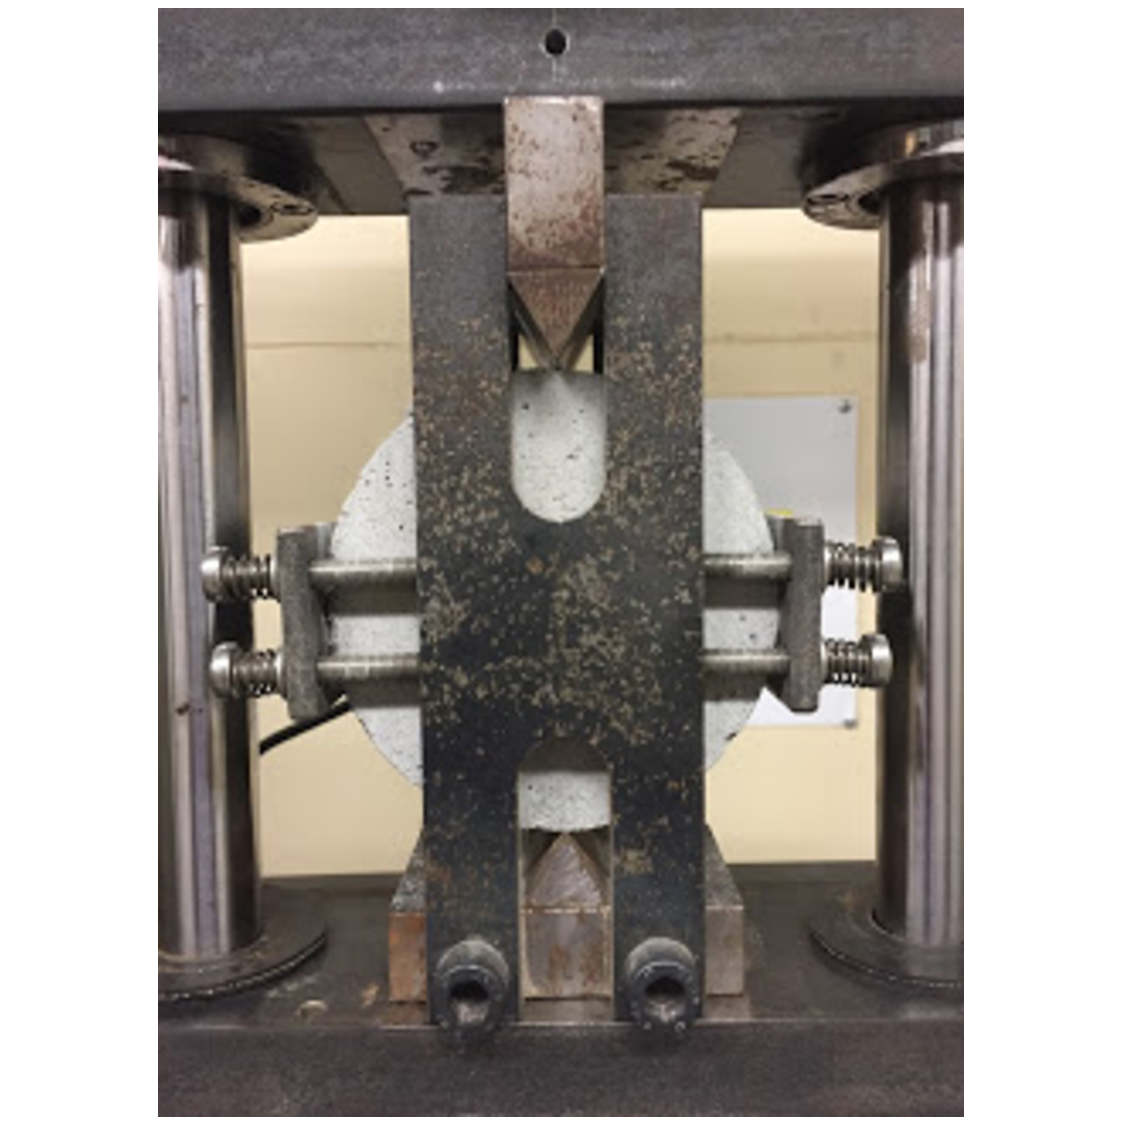
\includegraphics[width = \linewidth]{CR2}
			\caption{Splitting tensile test apparatus}
		\end{subfigure}
	\hspace{-0.1em}
		\begin{subfigure}{0.31\textwidth}
		\centering
		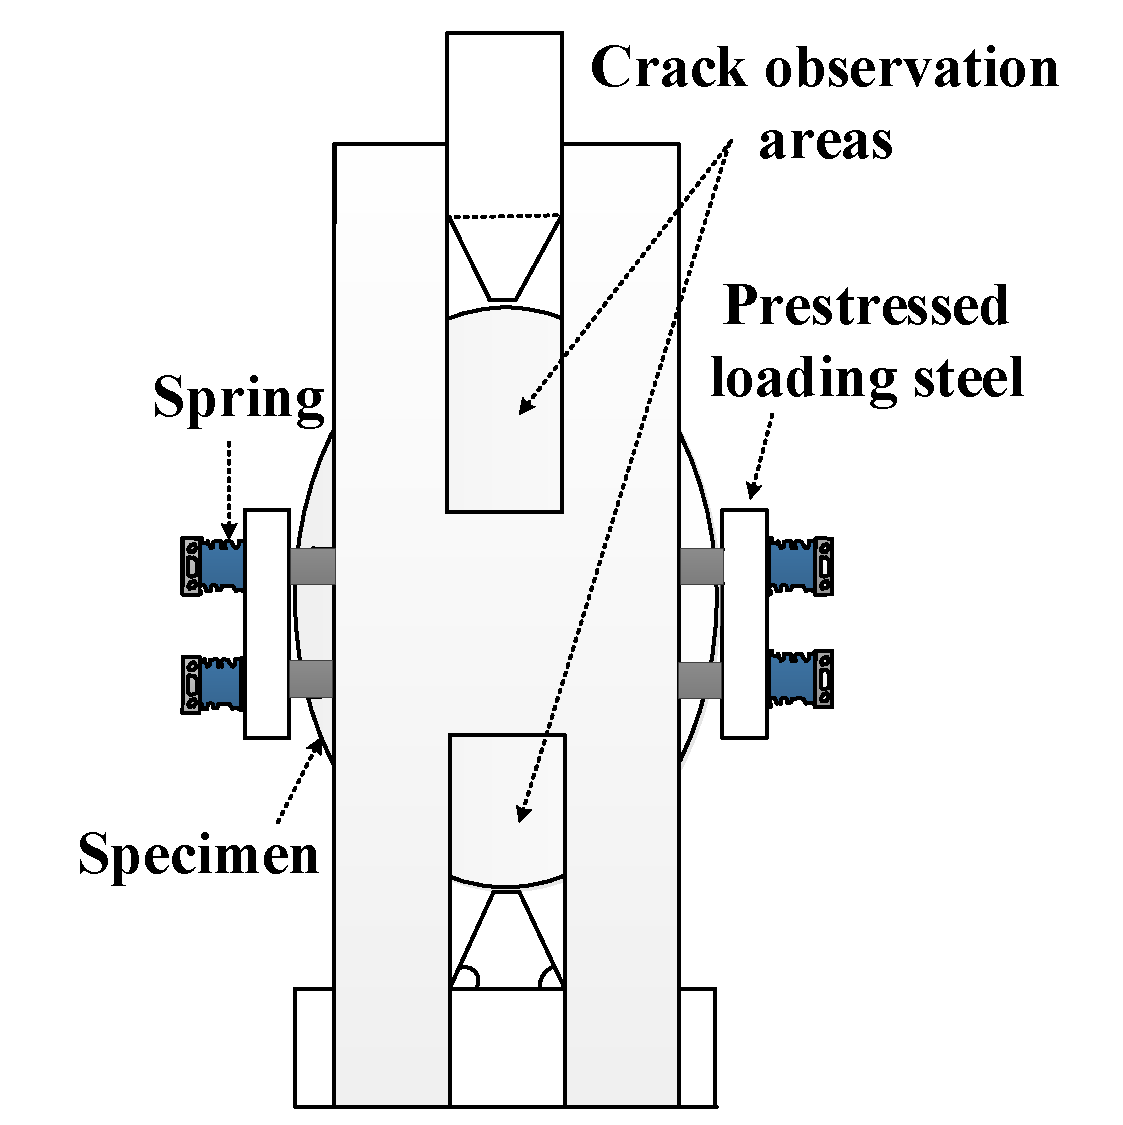
\includegraphics[width = \linewidth]{CR1}
		\caption{Schematic diagram of apparatus}
		\end{subfigure}	
	\hspace{-0.10em}
		\begin{subfigure}{0.31\textwidth}
		\centering
		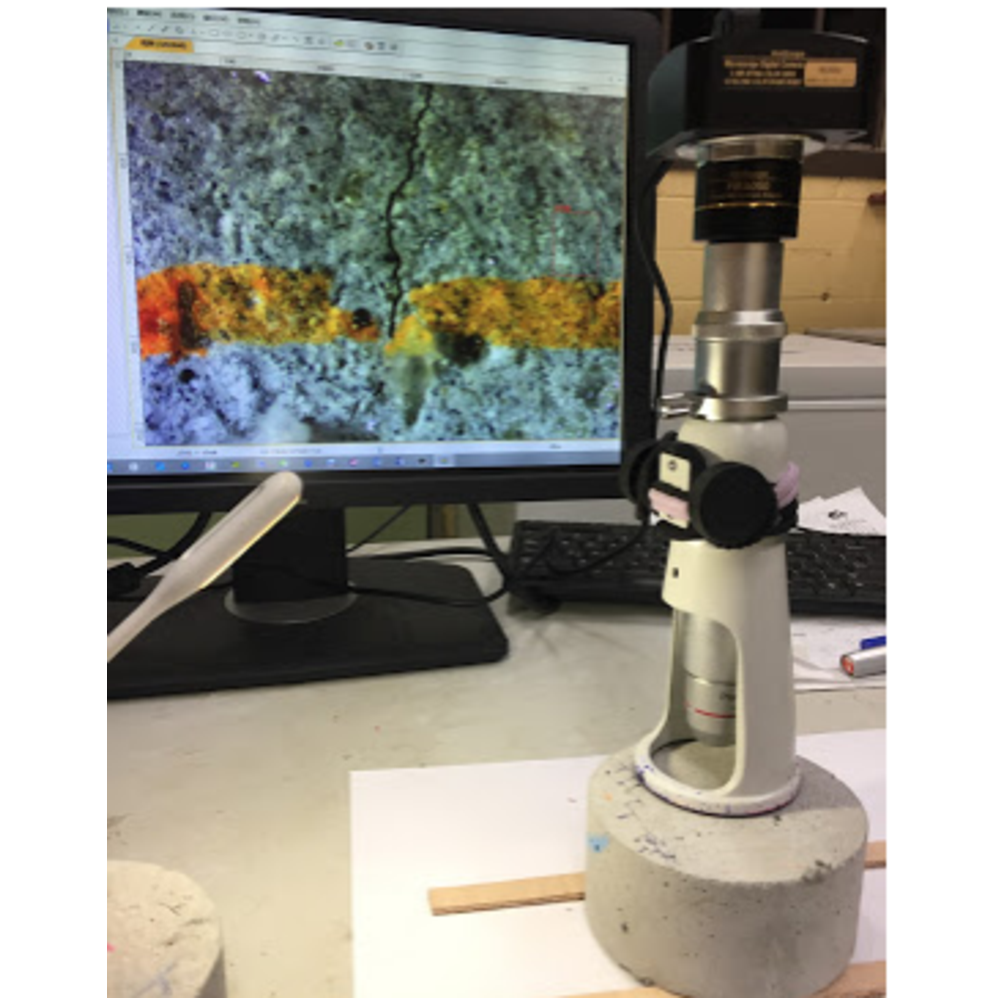
\includegraphics[width = \linewidth]{CR3}
		\caption{Crack width measurement}
		\end{subfigure}
		\caption{Splitting tensile test apparatus and microscope used in experiment for creating and measuring ECC cracks}\label{f:cr1}
	\end{figure}
	
	Micro-cracks less than $150 \mu m$ were first produced by pre-loaeding up to 70\% of their maximum splitting strength. We used a digital microscope to observe the crack width on the surface of specimens shown in Figure \ref{f:cr1} (c). After that, specimens were subjected to self-heal through wet-dry (W/D) cycles which contained submersion in water at $23 \pm 2^\circ C$ for 24 hours and drying in a laboratory medium at $50 \pm 5\%$ RH and $23 \pm 2^\circ C$ for 24 hours. After 10 W/D cycles, cracks are measured again by the digital microscope to indicate the partial or full closure of crack. Figure \ref{f:cr2} illustrated the comparison of crack width changes for two ECC mixture specimens before and after W/D cycles due to self-healing. 

	
	\begin{figure}[!h]
	\centering
	\begin{subfigure}{0.3\textwidth}
		\centering
		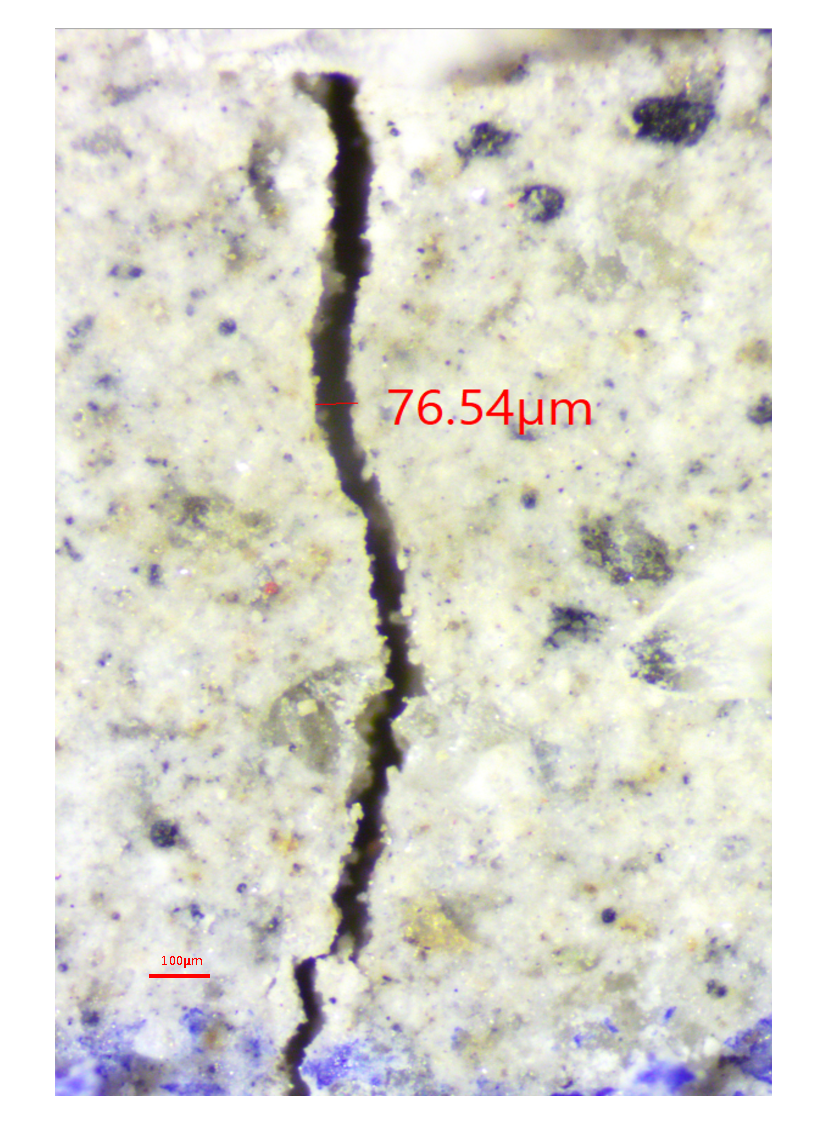
\includegraphics[width = \linewidth]{crack11}
		\caption{S1: crack before self-healing}
	\end{subfigure}
	\hspace{1em}
	\begin{subfigure}{0.3\textwidth}
		\centering
		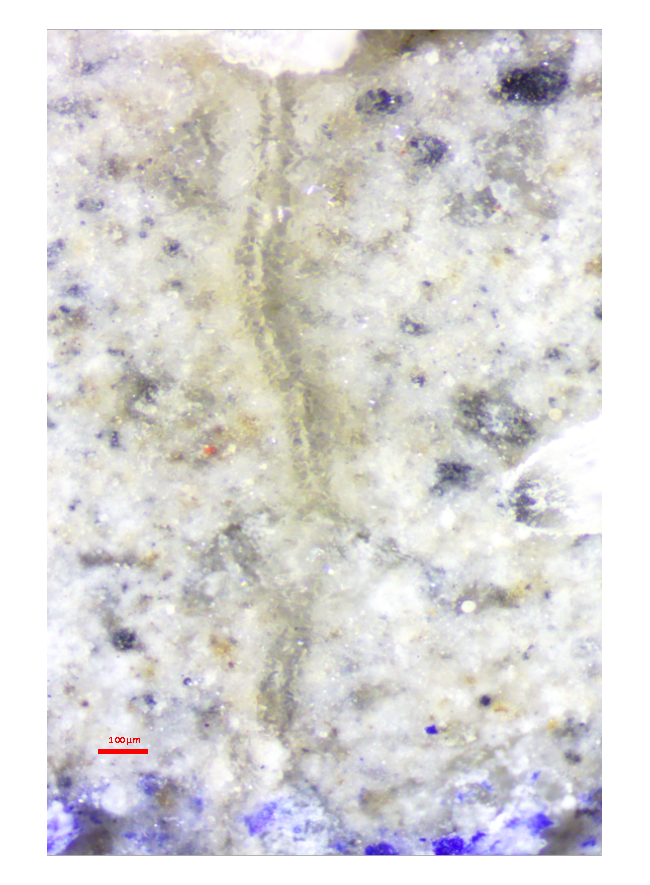
\includegraphics[width = \linewidth]{crack1}
		\caption{S1: crack after self-healing}
	\end{subfigure}	
%		\subfigure[]{%
%			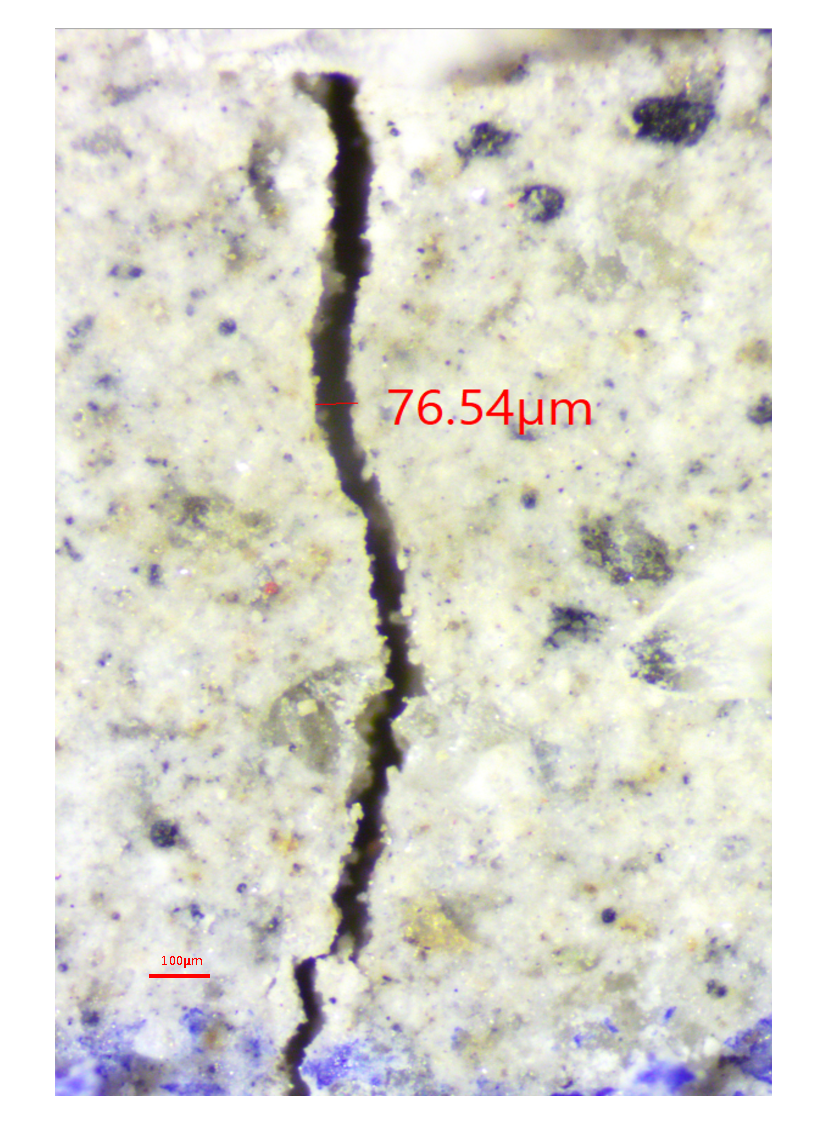
\includegraphics[width=.25\textwidth]{crack11}}\hfill
%		\subfigure[]{%
%			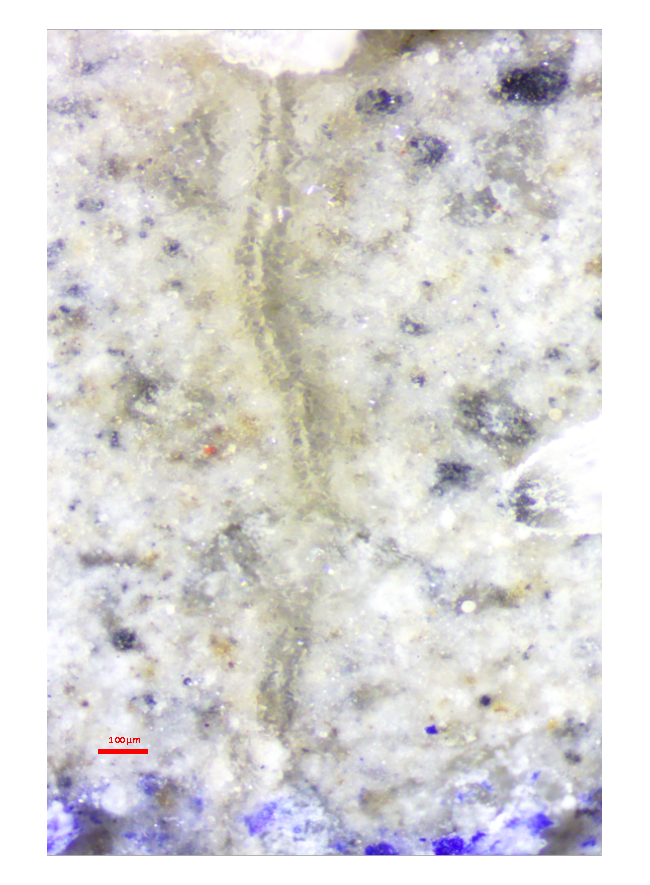
\includegraphics[width=.25\textwidth]{crack1}}\hfill
%		\subfigure[S2: crack before self-healing]{%
%			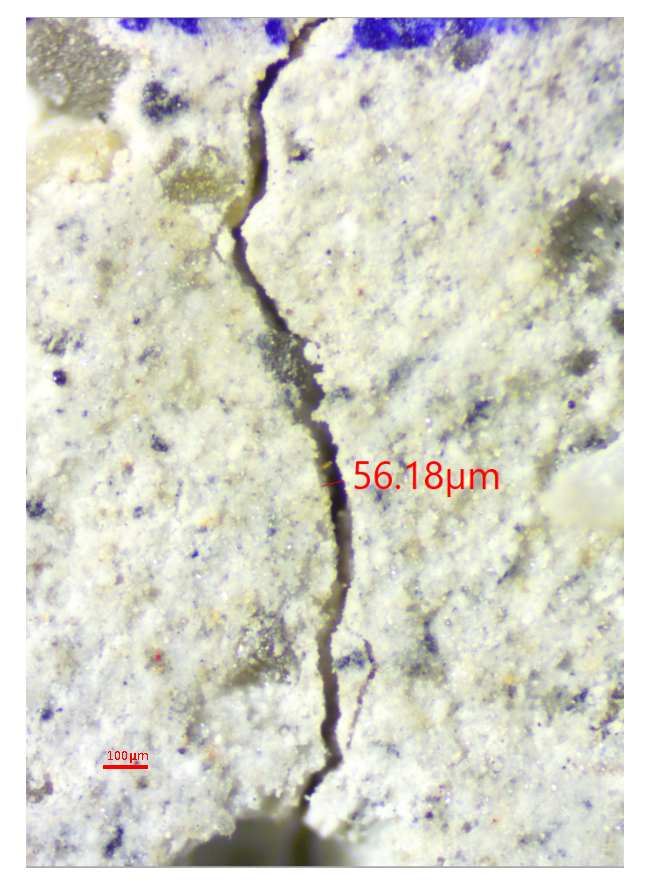
\includegraphics[width=.25\textwidth]{crack2}}\hfill
%		\subfigure[S2: crack after self-healing]{%
%			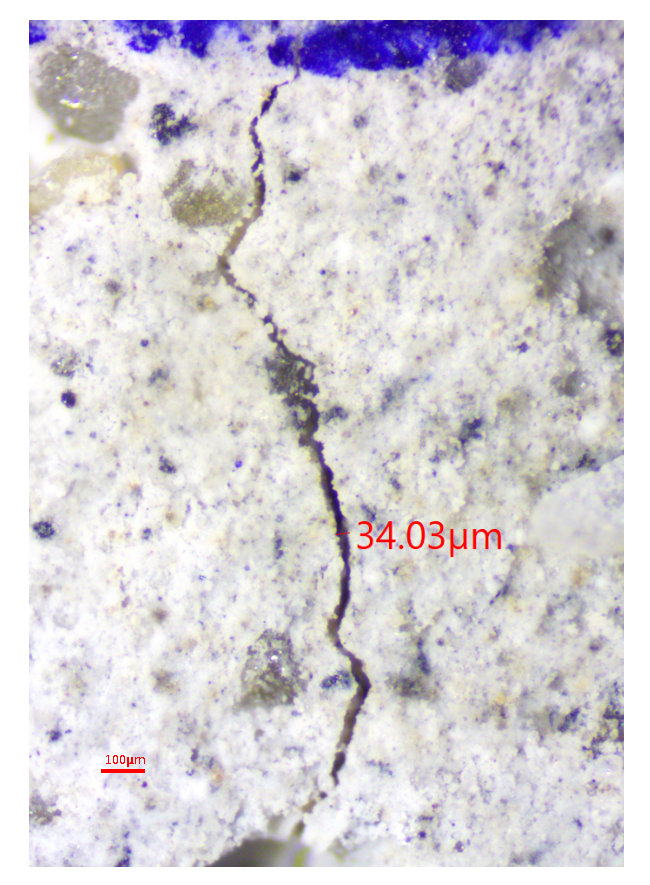
\includegraphics[width=.25\textwidth]{crack22}}\hfill
		\caption{Comparison of crack width changes in two ECC specimens, S1 and S2, before and after self-healing}\label{f:cr2}
	\end{figure}
	
	
%\subsection{The quantitative definitions for self-healing of ECC}
%
%To define the self-healing ability of ECC quantitatively, the crack width before  
%		
		
	\subsection{Data Collection}
	\label{dc}
	
	\begin{figure}[!h]
		\centering
		\includegraphics[width=.75\textwidth]{measurement}
		\caption{Schematic diagram of measuring observation areas on the surface of ECC mixture specimen}
		\label{ma}
	\end{figure}
	
	
	Empirical data for prediction were gathered with four features, crack width before self-healing representing the influencing factor of self-healing, and the weight of FA, SF, and LP illustrating the variable composites of ECC. It is noteworthy that some impact factors in the test, such as GPC, sand, W/CM, and healing time are controlled as constants which are excluded for the prediction modeling due to no effect. There are 6 specimens with dimension of $\O 50mm \times 100mm$ for each mixtures which were observed using digital microscope to collect crack width samples before self-healing and after self-healing. Four horizontal lines were drawn on the surface of each specimen along the direction of vertical force, which divided the specimen into five observation areas. The schematic diagram of observation measurement is shown in Figure \ref{ma}. In each observation area, we recorded one data sample if the crack width showed little change along the vertical force; Otherwise, we recorded multiple data samples with different crack widths separately before and after self-healing, while the crack width is inconsistent along the vertical force. For example, the front end of the crack is wide, and the rear part is narrow. Totally, 617 data samples were collected from nine mixtures to construct machine learning training-testing dataset. Table \ref{min} shows the number of collected samples and range of crack width before and after self-healing in each mixture. 
	

	\begin{table}[!h]
		\centering
		\caption{Number of crack samples and range of crack width before and after self-healing collected from nine ECC mixes}
		\label{min}
		\begin{tabular}{p{1.02in}p{1.2in}cccc}
			\toprule
			&		&	\multicolumn{2}{p{1.9in}}{Crack width before self-healing}	&	\multicolumn{2}{p{1.8in}}{Crack width after self-healing}	\\ \cmidrule(r){3-6}
			Mix	&	Number of crack samples	&	Min	($\mu m$) &	Max ($\mu m$)	&	Min ($\mu m$)	&	Max ($\mu m$)	\\
			\midrule
			FA70	&	87	&	3.28	&	134.69	&	0	&	121.37	\\
			FA65-SF5	&	77	&	4.37	&	135.47	&	0	&	124.01	\\
			FA60-SF10	&	88	&	5.18	&	121.78	&	0	&	113.11	\\
			FA55-SF15	&	88	&	3.45	&	115.8	&	0	&	109.53	\\
			FA65-LP5	&	112	&	7.65	&	119.45	&	0	&	105.65	\\
			FA60-LP10	&	37	&	5.62	&	126.82	&	0	&	110.97	\\
			FA55-LP15	&	61	&	6.42	&	132.65	&	0	&	115.95	\\
			FA55-SF5-LP10	&	34	&	8.74	&	123.09	&	0	&	110.78	\\
			FA55-SF10-LP5	&	33	&	4.64	&	131.57	&	0	&	119.79	\\
			%Total	&	617	&	-	&	-	&	-	&	-	\\
			\bottomrule
		\end{tabular}
	\end{table}
	

	
	\subsection{Preprocessing of Data}
	
	The input and output data of different features (referring to Table \ref{mx} and \ref{min}) vary in range and units which weigh all features unequally for prediction models and might end up creating bias. To eliminate this effect, we preprocessed empirical data to the range [0,1] by the min-max scaling presented in the following function. 
	
	\begin{equation}
	x' = \frac{x - x_{min}}{x_{max} - x_{min}}
	\end{equation}
	
	
	Where $x'$ is the scaled value of the variable $x$, $x_{max}, x_{min}$ are the maximum and minimum values of variable $x$ respectively. 
	

	
	%%%%%%%%%%%%%%%%%%%%%%%%%%%%%%%%%%%%%%%%%%
	
	
	\section{Methodology}
	\label{meth}
	
	Machine learning techniques used to predict the self-healing capability of ECC in this study are four individual methods including LR, SVR, BPNN and CART, as well as three ensemble methods including bagging, AdaBoost and stacking. Ensemble methods are constructed using individual methods as base estimators to predict the self-healing capability of ECC. To establish a baseline for comparison, modeling parameters of individual methods are set to the same in both individual models and ensemble models. The reason of choosing these techniques are because they are the most popular, and some of are even recognized as the top data mining algorithms in related field of concrete \cite{chou2014machine}. The proposed individual and ensemble techniques are described in the following subsections. 
	
	
	\subsection{Linear Regression}
	
	LR attempts to determine the relationship between a dependent variable (response variable) and one or more independent variables (explanatory variables) by fitting a linear regression equation \cite{neter1996applied}. Given our dataset $T = \{ (x_i,y_i), i = 1,2,...,n\}$, where $n = 617$ is the size of sample dataset. $x_i \in R^n$ is independent variables representing a sample of selected features from FA, SF, LP and crack width before self-healing, $R^n$ is $n$-dimensional space, $y_i \in R^1$ is the target output (crack width after self-healing) that corresponds to $x_i$. Let $d = 4$ denote the number of a independent variable  of an random vector $x = \{ x_1;x_2;...;x_d \}$, and $y$ is the corresponding output ( dependent variable). The general formula of LR for predicting self-healing capability of ECC can be expressed as follows:
	
	\begin{eqnarray}
	y = w_1 x_1 + w_2 x_2 + ......+ w_d x_d +b                                                      
	\end{eqnarray}
	where $w_i, (i = 1,2,...,d)$ denotes a regression coefficient, $b$ is an error term. 
	
	\subsection{Support Vector Regression}
	
	The support vector machine (SVM) is a supervised machine learning method and first introduced by Vapnik \cite{cortes1995support,vapnik1999overview} based on statistical learning theory \cite{juncai2015prediction}. Since then, it gains popularity due to attractive features, and promising empirical performance. SVM includes two main categories: support vector classification (SVC) and SVR. For classification problem, input data as vectors are mapped to a high-dimension feature space where an optimal separating hyperplane is constructed by using a \textit{kernel} function to assign new data into different categories\cite{suykens1999least}. By implementing the structural risk minimization (SRM), SVC obtains good generalization. 
	
	For the regression, the basic idea is to provide a nonlinear function by mapping input data into the high-dimensional feature space where a special type of hyperplane is constructed. After that, a regression model is build in the hyperplane \cite{li2007consensus}. It implements approximately the SRM to set up an upper bound of the generalization error so as to achieve generalized performance \cite{fang2008hybrid}.
	
	Given our dataset $T = \{ (x_i,y_i), i = 1,2,...,n\}$, where $n = 617$ is the size of sample dataset, $x_i \in R^n$ is the input vector representing a sample of selected features from FA, SF, LP and crack width before self-healing, $R^n$ is $n$-dimensional vector space, $y_i \in R^1$ is the target output indicating crack width after self-healing  that corresponds to $x_i$. The SVR aims to seek a optimum regression function $f(x)$ with minimized empirical risk, which can be expressed as follow:
	
	\begin{eqnarray}
	f(x) = \langle w,x \rangle + b \quad \text{with} \quad w \in T, b \in R                                                              
	\end{eqnarray}
	where $\langle \cdot, \cdot \rangle$ denotes the dot product in $T$, $w$ and $b$ are the weight vector and bias value which are estimated by minimizing the empirical risk, that is, the distance between the predicted crack width and the target crack width after self-healing.  
	
	SVR adopts an $\epsilon$-insensitive loss function penalizing predictions that has a distance between the predicted crack width and the target crack width after self-healing greater than $\epsilon$.  Therefore, the problem of finding $w$ and $b$ to reduce the empirical risk with respect to an $\epsilon$-insensitive loss function is equivalent to the convex optimization problem that minimizes the margin ($w$) with the full prediction error within the range of $\epsilon$. Then this problem can be expressed as: 
	%:
	\begin{eqnarray} \label{svr2}
	\begin{aligned}
	\text{minimize} \quad& \frac{1}{2} ||w||^2 \\
	\text{subject to} \quad & 
	\left  \{ 
	\begin{array}{l}
	y_i -\langle w,x_i \rangle -b \le \epsilon \\
	\langle w,x_i \rangle +b -y_i \le \epsilon
	\end{array}
	\right.
	\end{aligned}                                                            
	\end{eqnarray}
	By introducing slack variables $\xi, \xi_i^*$ to allow some errors to cope with infeasible solution of the optimization problem, the formulation can be generated as \cite{vapnik1999overview}: 
	
	\begin{eqnarray}
	\begin{aligned}
	\text{minimize} \quad &  \frac{1}{2} ||w||^2 + C \sum_{i=1}^{n}(\xi + \xi_i^*) \\
	\text{subject to} \quad& 
	\left \{
	\begin{array}{l}
	y_i - \langle w, x_i \rangle -b \le \epsilon + \xi_i \\
	\langle w, x_i \rangle + b - y_i \le  \epsilon + \xi_i^* \\
	\xi_i, \xi_i^* \ge 0 
	\end{array}
	\right.
	\end{aligned}                                                              
	\end{eqnarray}
	
	The constant $C$  is the penalty value imposed on predictions that lie outside the $\epsilon$ margin. After calculating a Lagrange constructed from objective function and all constraints, introducing a dual set of variables as follows \cite{yuvaraj2013support}:
	\begin{eqnarray}
	\begin{aligned}
	L_P  = & \frac{1}{2} ||w||^2 +C\sum_{i=1}^{n} (\xi_i + \xi_i^*) - \sum_{i=1}^{n} (\eta_i \xi_i + \eta_i^* \xi_i^*) \\
	& -\sum_{i=1}^{n} \alpha_i (\epsilon + \xi_i - y_i + \langle w, x_i \rangle + b) \\
	& - \sum_{i=1}^{n} \alpha_i^* (\epsilon + \xi_i^* +y_i - \langle w, x_i \rangle -b )
	& \\
	s.t. \quad & \alpha_i, \alpha_i^*, \eta_i, \eta_i^* \ge 0 
	\end{aligned}.                                                               
	\end{eqnarray}
	
	Where $L_P$ is the Lagrangian and $ \alpha_i, \alpha_i^*, \eta_i, \eta_i^* $ are Lagrange multipliers.
	
	The optimality can be achieved by the partial derivatives of $L_P$ with respect to the primal variables following the saddle point condition. Then the function of SVR is obtained as:
	\begin{eqnarray}\label{svr3}
	f(x) = \sum_{i=1}^{n} (\alpha_i - \alpha_i^*)\langle x_i , x \rangle +b                                                             
	\end{eqnarray}
	
	As for the nonlinear regression, the input data have to be mapped into a high-dimensional feature space, in which dot product can be replaced by a kernel function $k(x_i, x_j) = \phi(x_i)^T\phi(x_j)$, and the function \eqref{svr3} can be written as:
	\begin{eqnarray}
	f(x) = \sum_{i=1}^{n}(\alpha_i - \alpha_i^*)k(x_i , x) +b                                                          
	\end{eqnarray}
	
	
	There are various kernel functions, such as linear, polynomial, radial basis function and sigmoid kernel.  In this work, the Gaussian radial basis function (RBF) is chosen, which is defined as \cite{smola2004tutorial}: 
	\begin{eqnarray}
	k(x_i, x_j) = exp ({- \frac{||x_i -x_j ||^2}{2 \sigma^2} })                                                           
	\end{eqnarray}
	
	
	\subsection{Artificial Neural Network}
	Artificial neural network (ANN), also called neural network which is originated from simulating biological neural networks. Generally, it consists of many neurons in layers including one input layer, one or several hidden layers and an output layer \cite{mukherjee1997artificial}. The neurons are fully interconnected between the neighboring layers by weight, and typically no inter-connections between neurons within the same layer \cite{naderpour2018compressive}. 
	
	There are many possible network structures, in this study the type utilized is the BPNN. A preliminary architecture of the BPNN is determined to be 4 - $n$ - 1, where 4 input neurons represent the input features standing for FA, LP, SF and crack width before self-healing, $n = 5$ indicates the number of neurons in the hidden layer, and 1 target neuron in the output layer for the predicted crack width after self-healing. This is a three-layer network with one hidden layer which is already able to approximate most continuous function, of which the complex nonlinear relationship could be approximated in accuracy \cite{yan2017evaluation}. The architecture of the BPNN model for predicting self-healing is demonstrated in Figure \ref{fig:BPNN}. %Details of input parameters see in Section \ref{experi} and \ref{dc}.
	
	\begin{figure}[!]
		\begin{center}
			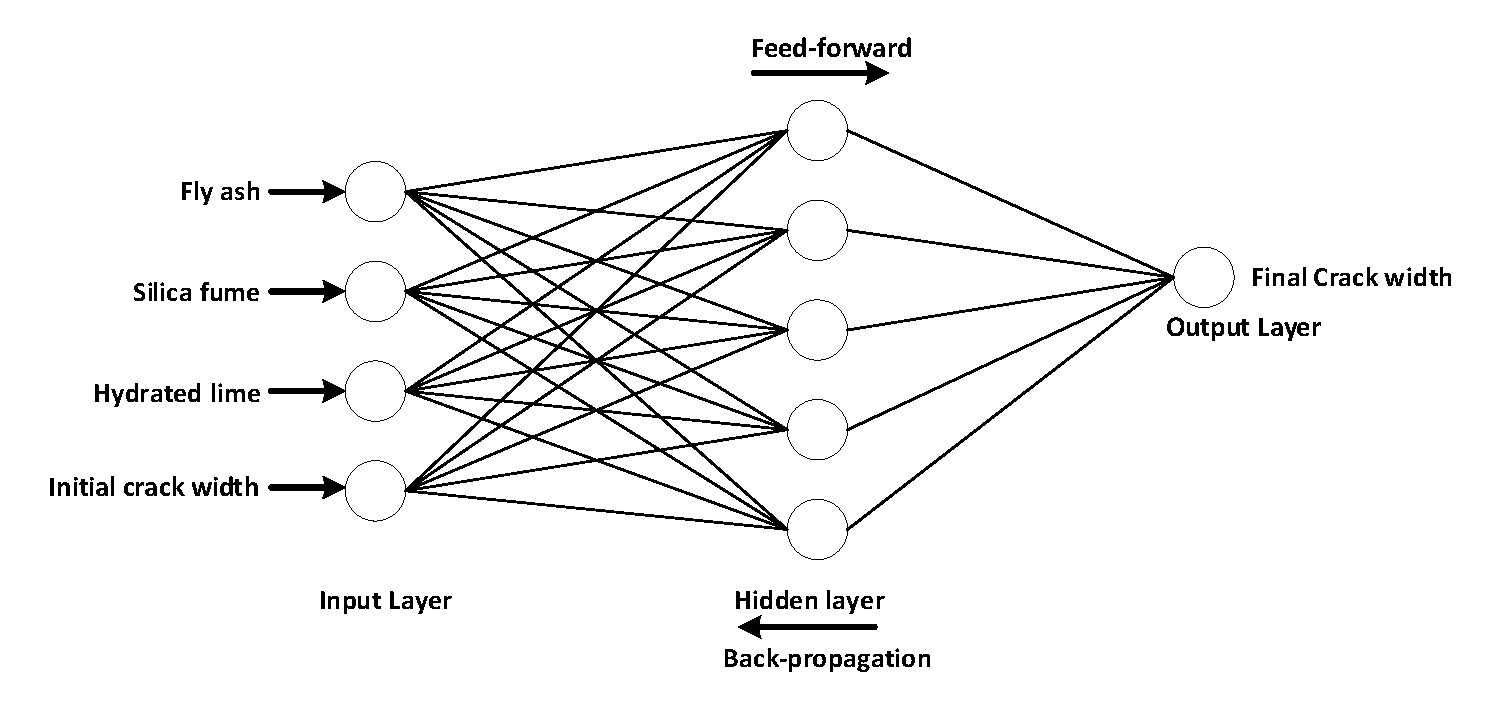
\includegraphics[width=\textwidth]{BPNN.pdf}
		\end{center}
		\caption{Schematic diagram of BPNN model for predicting self-healing capability of ECC}
		\label{fig:BPNN}
	\end{figure}
	
	Given a set of inputs $ \{ x_1, x_2,x_3,..., x_n\}$, while information is passed through the input layer to the hidden layer, each neuron in the input layer are multiplied by respective weights added by a bias and are summed together. After that, a activation function $f$ is applied to form the output $z$. This can be expressed in the following equation \cite{alshihri2009neural}:
	
	\begin{equation}
	z = f(\sum_{i=1}^{n} w_{ij}x_i + b_j)
	\end{equation}
	
	where $w_{ij}$ is the connection weights between the $i$th neuron of input and the $j$th neuron in the hidden layer, and $b_j$ is the bias of the $j$th neuron. The sigmoid function is applied as activation function between the input, hidden, and output neurons to form the output. 
	
	\begin{equation}
	f(x) = \frac{1}{1+e^{-x}}
	\end{equation}
	
	The goal of training a neural network is to determine the values of the connection weights and the biases of the neurons. The back propagation indicates a iterated method which adjusts the weights from output layer to input layer. At first, a output are calculated feed-forward from the input layer via the hidden layer to the output layer. Then a error is generated by comparing the output with the target output. After that, the error is back propagated to the hidden layer and input layer with adjusting the connection weights and biases to reduce the error. Such a process will be repeated until the error is minimized or the termination is reached to avoid over-fitting. 
	
	
	
	\subsection{Classification and Regression Tree}
	
	The CART \cite{breiman2017classification}  is a tree decision algorithm that split data into mutually exclusive subgroups based on recursive binary partitioning procedure. It develops the relationship between the target variables (the crack width after self-healing of ECC) and the independent variables (the input features of FA, SF, LP and crack width before self-healing of ECC) to create decision rules to form subgroups as branches and leaves in the Figure \ref{fig:CART} that illustrates the schematic diagram of a decision tree. The process of CART starts from the root node which contains the entire data set to construct two sub-nodes representing two categories. Then this recursion process is applied to each sub-node until all divided sub-nodes are leaf nodes. The CART tree can be either a classification tree \cite{dan1995cart} or regression tree \cite{put2003classification} depending on the type of target and independent variables which may be categorical or numerical. 
	
	\begin{figure}[!htb]
		\begin{center}
			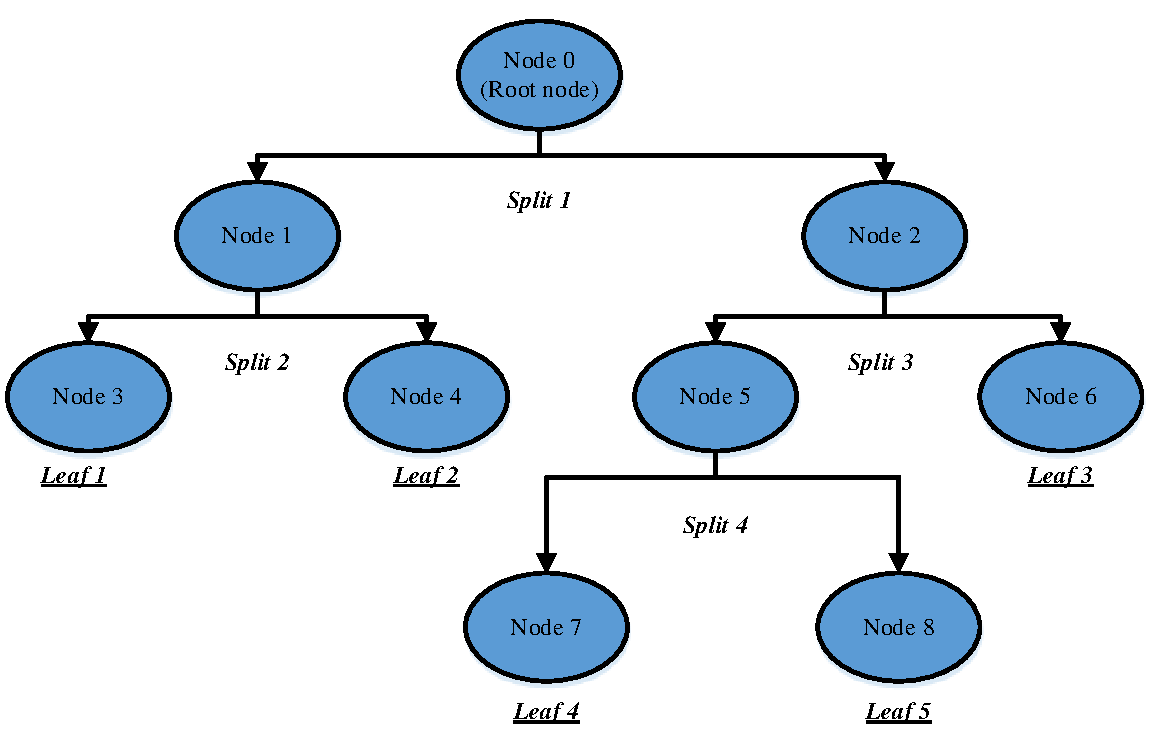
\includegraphics[width=0.75\textwidth]{CART}
		\end{center}
		\caption{Structure of a classification and regression tree \cite{put2003classification}}
		\label{fig:CART}
	\end{figure}
	
	
	The key idea of constructing a CRAT tree is achieved by selecting a variable at each node that best splits the empirical data. To locate splits, $Gini$ index is used to measure the impurity of the two child nodes which contains subsets of data are as homogeneous as possible with respect to the target variable.  
	
	Given a dataset has $K$ classes and probability of a sample which belongs to class $i$ is $p_i$, $i \in \{1,2,3,...,K\}$, the $Gini$ impurity can be expressed as,
	
	\begin{equation}
	G(p) = \sum_{i=1}^{K}p_i(1-p_i) = 1- \sum_{i=1}^{K}p_i^2
	\end{equation}
	
	
	\subsection{Ensemble Methods}
	
	In contrast to various learning approaches such as SVM, CART which develop a single learner from training data, ensemble methods train multiple base learners and combine them \cite{chou2014machine} to improve generalizability over a single estimator. Therefore, weak learners (base learners) can be boosted to strong learner \cite{frosyniotis2003divide} in a ensemble method. The set of base learners in an ensemble are developed from a individual learning algorithm which can be decision tree, SVM, or other kinds of learning algorithms. Researches \cite{dietterich2000ensemble} show that ensemble methods are usually significantly more accurate than individual learning methods  
	
	Suppose with a $d$-dimensional predictor variable $X$ (input features of FA, SF, LP, and crack width before self-healing of ECC) and one dimensional output $Y$ (The crack width after self-healing of ECC). Each estimator uses a individual algorithm to provide one estimated function $g(\cdot)$. The output presented by ensemble-based function $g_{en}(\cdot)$ is obtained by a linear combination of individual functions. This ensemble approach can be expressed mathematically as:
	
	\begin{equation}
	g_{en}(\cdot) = \sum_{j=1}^{N}c_j *g(\cdot)
	\end{equation}
	
	Where $c_j$ expresses the combination coefficients which is dependent on the used ensemble models.  
	
	\subsubsection{Bagging}
	
	Bagging (bootstrap aggregating) generate multiple versions of a predictor to obtain an aggregated predictor \cite{breiman1996bagging}. It generates multiple models independently on different versions of data set which are random bootstrap replications of original training set. That is, several training examples may repeatedly appear in different bootstrap replicated data set. Then those individual predictions are aggregated through an combination method (either voting or averaging) to form the final prediction. By introducing randomization into bagging method's construction procedure and making an ensemble out of it, bagging method is used as a approach to reduce the variance of a base estimator, such as a regression tree. 
	
	% In many cases, bagging methods constitute a very simple way to improve with respect to a single model, without making it necessary to adapt the underlying base algorithm.
	
	\subsubsection{AdaBoost}
	
	Liking bagging, AdaBoost \cite{freund1996experiments} manipulates modified versions of training examples repeatedly to generate multiple predictions which are then combined to form the final prediction. The difference is that AdaBoost applies a weight to each of the training examples. In each iteration, the weights are individually updated based on minimizing the weighted error on the training set. It increases weights on those training examples were incorrectly predicted in previous iteration by the boosted model, whereas the weights are decreased for correctly predicted training examples. In subsequent iterations, therefore, AdaBoost constructs progressively more difficult learning problems.  Once the training process has finished, the predictions are combined through a weighted majority vote (or sum) to produce the final prediction. The final classifier therefore usually achieves a high degree of accuracy in the test set.
	
	\subsubsection{Stacking}
	
	Stacking regression combines multiple regression models via a meta-regression, which use out-of-fold predicts concept \cite{raschkas_2018_mlxtend} (Shown in Figure \ref{fig:Stack}). It split the data set into K folds, k-1 folds are used to train the first level regressors in K successive rounds. In each round, the first level regressors are used to predict based on the remaining 1 subset. After that, the prediction results is used and stacked as input data to the second level regressor to form a final set of predictions \cite{sill2009feature}. In this study, SVR, BPNN and CRAT are used as regression models in the first level to get prediction results, and LR is used as met-regressor in the second level to combine and generate final prediction. 
	
	
	\begin{figure}[!h]	
		\begin{center}
			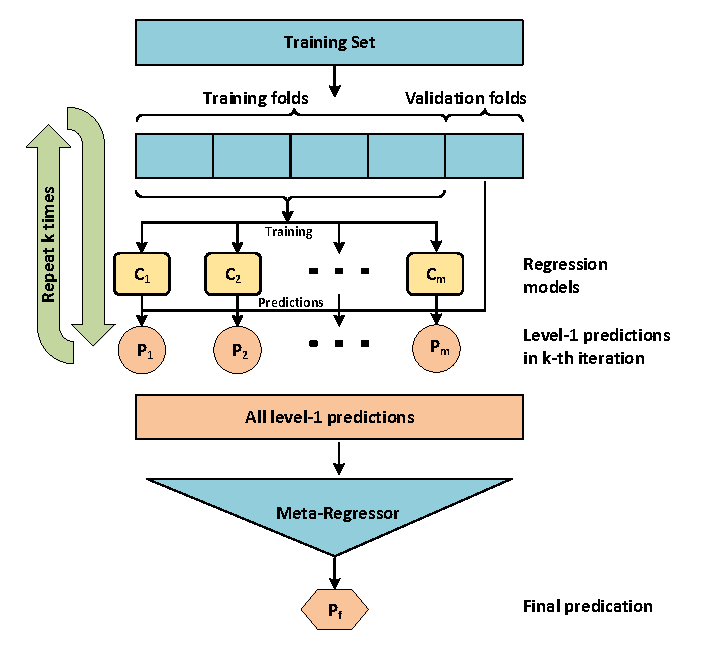
\includegraphics[width=0.75\textwidth]{SP}
		\end{center}
		\caption{Schematic diagram of Stacking model \cite{sill2009feature}}
		\label{fig:Stack}
	\end{figure}
	
	
	
	%%%%%%%%%%%%%%%%%%%%%%%%%%%%%%%%%%%%%%%%%%
	
	
	%%%%%%%%%%%%%%%%%%%%%%%%%%%%%%%%%%%%%%%%%%
	\section{Validation and Evaluation}
	\label{4}
	
	
	
	\subsection{Cross-validation Method}
	\label{cross}
	Generally, dataset is split to generate a training subset and a validation subset keeping the properties of the original dataset as much as possible to avoid misleading estimates. To minimize bias of random data splitting, the K-fold cross-validation is used widely \cite{chou2014machine}. In this study. a ten-fold cross-validation approach is applied to assess model performance in this study (shown in Figure \ref{fig:TFC}), which yields the optimal computational time and reliable variance confirmed by Kohavi \cite{kohavi1995study}. The empirical dataset is split into 10 equal-size subsets with a similar distribution. After that, training-tests perform repeatedly for 10 times using a different subset as the test set and the remaining subsets as the training set in each time \cite{dor2007achieving}. The average accuracy in 10 times validation is expressed as the model accuracy.
	
	\begin{figure}[!h]
		\begin{center}
			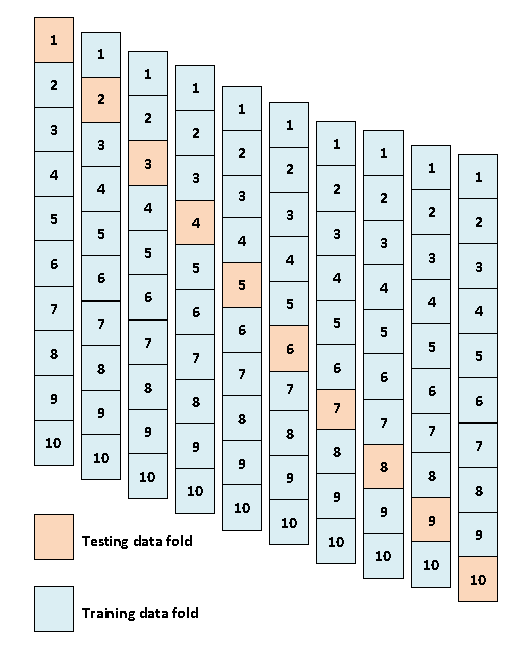
\includegraphics[width=0.65\textwidth,height=0.65\textwidth]{TC}
		\end{center}
		\caption{Ten-fold cross-validation approach}
		\label{fig:TFC}
	\end{figure}
	
	\subsection{Performance Evaluation}
	
	To indicate and validate the accuracy of proposed machine learning models, three statistical indices, mean absolute Error (MAE), root mean square error (RMSE), and the coefficient of determination $R^2$ are used as the following equations. The average deviation of the performance of a individual model or an ensemble model from a benchmark model in terms of  three statistical measures (MAE, RMSE and  $R^2$) is calculated following  equation (\ref{CP}).	
	
	\begin{itemize}
		\item Mean absolute error (MAE). 
		\begin{eqnarray}
		MAE = \frac{1}{n}\sum_{i=1}^{n}{|y_i - y_i^{'}|}                                                       
		\end{eqnarray}
		\item Root mean square error (RMSE)
		\begin{eqnarray}
		RMSE = \sqrt{\frac{1}{n}\sum_{i=1}^{n}({{ y_i  - y_i^{'}}} )^2}                                                         
		\end{eqnarray}
		\item Coefficient of determination ($R^2$)
		\begin{eqnarray}
		R^2 = 1 - \frac{\sum_{i=1}^{n}(y_i - y_i^{'})^2}{ \sum_{i=1}^{n} (y_i -\overline{y})^2  }                                             
		\end{eqnarray}
		\item Deviation ($Dev$)
		\begin{equation}
		\label{CP}
		Dev(\%) = \frac{P_i - P_{j}}{ P_{j}} * 100
		\end{equation}	
	\end{itemize} 
	
	Where $y_i$ is the target output, $y_i^{'}$ is the predicted output, $n$ is the number of samples, $\overline{y}$ is the mean of the target output. $Dev$ indicates the statistical performance improvement compared with a benchmark model, $P_i$ is the statistical performance (MAE, RMSE or  $R^2$) of an individual or ensemble method, $P_j$ is the corresponding performance of a benchmark model, LR or a individual method used in the ensemble method as the base learner, respectively.
	
	MAE statistics is a measure of errors between the predicted values (the estimated value of crack width of ECC after self-healing) with the estimated  values (the observed value of crack width of ECC after self-healing in empirical data). RMSE statistics computes the square root of the average residual error between the predicted values and the target values. A lower value of MAE or RMSE indicates a better prediction performance of the model. $R^2$ measures the strength of association between the predicted values and the target values, based on the proportion of total variation of outcomes. A greater value close to 1 represents a better prediction performance that commendably replicates the observed crack width of ECC after self-healing.  Deviation statistics indicates the improvement of the prediction performance of a individual or an ensemble model from a benchmark model that can be the LR model or the individual model used as base learners in the corresponding ensemble model. 
	
	
	
	%\begin{figure}[!h]
	%	\centering
	%	\includegraphics[width=0.9\textwidth]{01R2.png}
	%	\caption{Average $R^2$ results of all machine learning models on self-healing of ECC}
	%	\label{su}
	%\end{figure}
	
	%%%%%%%%%%%%%%%%%%%%%%%%%%%%%%%%%%%%%%%%%%
	\section{Results and Discussion}
	\label{result}
	
	In this section, the prediction performance of individual and ensemble methods are examined by MAE, RMSE and $R^2$ according to ten-fold cross-validation. Where we use the abbreviations for ease of presentation, in which Bag\_LR, Bag\_SVR, Bag\_BPNN and Bag\_CRAT express generating bagging ensemble method by using LR, SVR, BPNN and CRAT as base estimators, respectively. Ada\_LR, Ada\_SVR, Ada\_BPNN and Ada\_CRAT present generating AdaBoost ensemble method by manipulating LR, SVR, BPNN and CRAT as base estimators, respectively. Stack\_LR indicates developing stacking ensemble method based on individual methods (including SVR, BPNN, and CRAT) as learning base with using LR as a meta-regressor. 
	
	\subsection{Prediction performance of the proposed models}
	Table \ref{per} shows the average performance of ten-fold cross-validation for each model (in each row), and performance deviation from the LR model with respect of MAE, RMSE and $R^2$, respectively. As it can be seen, Stack\_LR is superior to all other individual or ensemble models on the basis of all three performance measures (3.934, 6.118, 0.904 for MAE, RMSE, and $R^2$, respectively). Furthermore, among the individual models, SVR performs the best in terms of MAE (4.296), and BPNN has the lowest error on RMSE (6.515) and highest accuracy with $R^2$ 0.899. For the single learning based ensemble methods, Bag\_CRAT has the best performance in terms of MAE (4.093), and Bag\_BPNN performs the best on RMSE (6.341). In terms of $R^2$, Bag\_CRAT and Bag\_BPNN have the same performance (0.901) and outperform other ensemble methods using an individual method as base estimator. Moreover, it can be concluded that most machine learning models are able to learn and predict empirical data with an acceptable degree of precision. The performance of all machine learning models described in Table \ref{per} are depicted in Figure \ref{comp} (a), (b), and (c) in terms of MAE, RMSE and $R^2$, respectively.
	
	\begin{table}[!h]
		\small
		\centering
		\caption{Average performances of machine learning models for self-healing prediction of ECC}
		\begin{tabular*}{0.75\textwidth}{ll|cc|cc|cc}
			\toprule
			&	Models	&	MAE	&	$Dev(\%)$	&	RMSE	&	$Dev(\%)$	&	$R^2$	&	$Dev(\%)$	\\
			%		&Models & MAE ($\mu m$) & $Dev$ (\%)  & RMSE ($\mu m$) & $Dev$ (\%) & $R^2$ & $Dev$ (\%)\\
			%		&  &  & LR  &  & LR  &  & LR  \\
			\midrule
			\multirow{4}{0.55in}{Individual models} &	LR	&	5.012	&	-	&	7.680	&	-	&	0.860	&	-	\\
			
			&	BPNN	&	4.329	&	-13.6	&	6.515	&	-15.2	&	0.899	&	4.5	\\
			
			&	CRAT	&	4.305	&	-14.1	&	6.811	&	-11.3	&	0.887	&	3.1	\\
			
			&	SVR	&	4.296	&	-14.3	&	6.826	&	-11.1	&	0.883	&	2.7	\\
			
			\midrule
			\multirow{10}{0.55in}{Ensemble models} 	&	Ada\_LR	&	4.784	&	-4.6	&	7.400	&	-3.6	&	0.867	&	0.8	\\
			
			&	Ada\_BPNN	&	4.226	&	-15.7	&	6.435	&	-16.2	&	0.900	&	4.7	\\
			
			&	Ada\_CRAT	&	4.207	&	-16.1	&	6.455	&	-15.9	&	0.898	&	4.4	\\
			
			&	Ada\_SVR	&	4.145	&	-17.3	&	6.577	&	-14.4	&	0.893	&	3.8	\\
			
			&	Bag\_LR	&	5.014	&	0.0	&	7.689	&	0.1	&	0.860	&	0.0	\\
			
			&	Bag\_BPNN	&	4.143	&	-17.3	&	6.341	&	-17.4	&	0.901	&	4.8	\\
			
			&	Bag\_CRAT	&	4.093	&	-18.3	&	6.358	&	-17.2	&	0.901	&	4.8	\\
			
			&	Bag\_SVR	&	4.302	&	-14.2	&	6.820	&	-11.2	&	0.883	&	2.7	\\
			
			&	Stack\_LR	&	3.934	&	-21.5	&	6.118	&	-20.3	&	0.904	&	5.1	\\
			\bottomrule
		\end{tabular*}
		\label{per}
	\end{table} 

\begin{figure}[!h]
		\centering
		\begin{subfigure}{.53\textwidth}
			\centering
			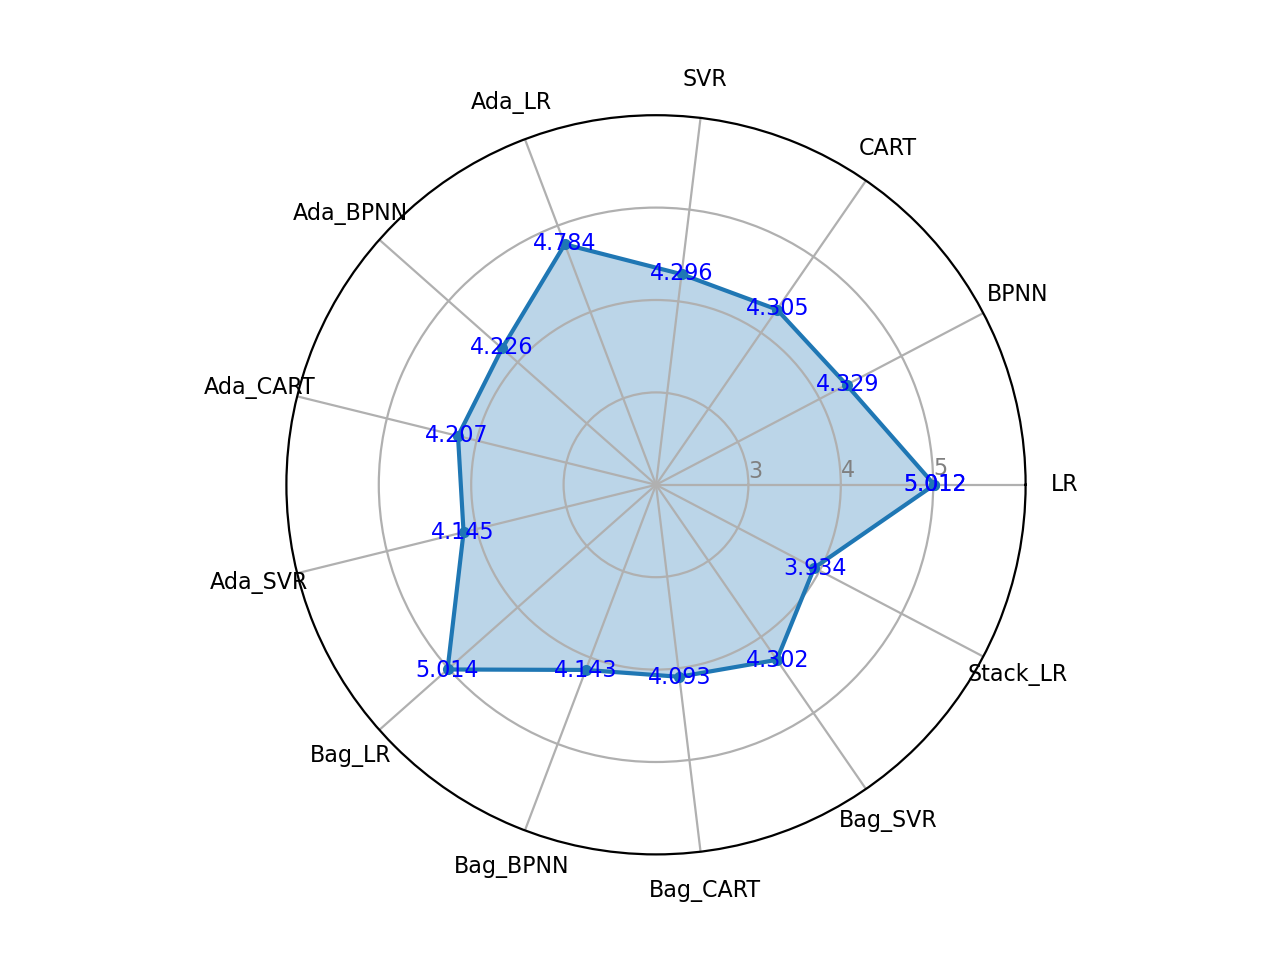
\includegraphics[width = \linewidth]{MAEcircle.png}
			\caption{MAE}
		\end{subfigure}%
		\hspace{-3em}
		\begin{subfigure}{0.53\textwidth}
		\centering
		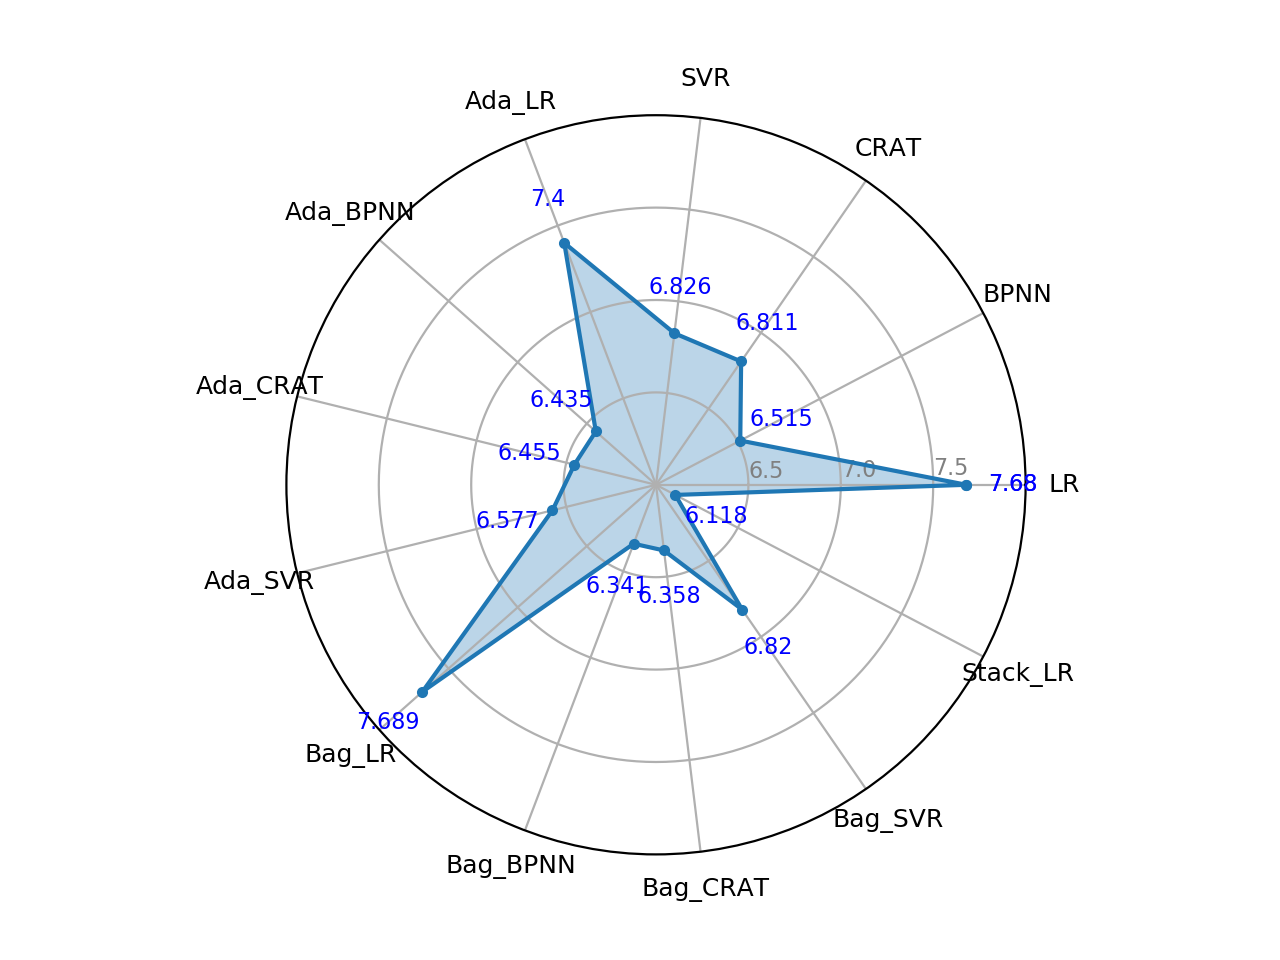
\includegraphics[width = \linewidth]{RMSEcircle.png}
		\caption{RMSE}
		\end{subfigure}%
		\hspace{1em}
		\begin{subfigure}{.53\textwidth}
			\centering
			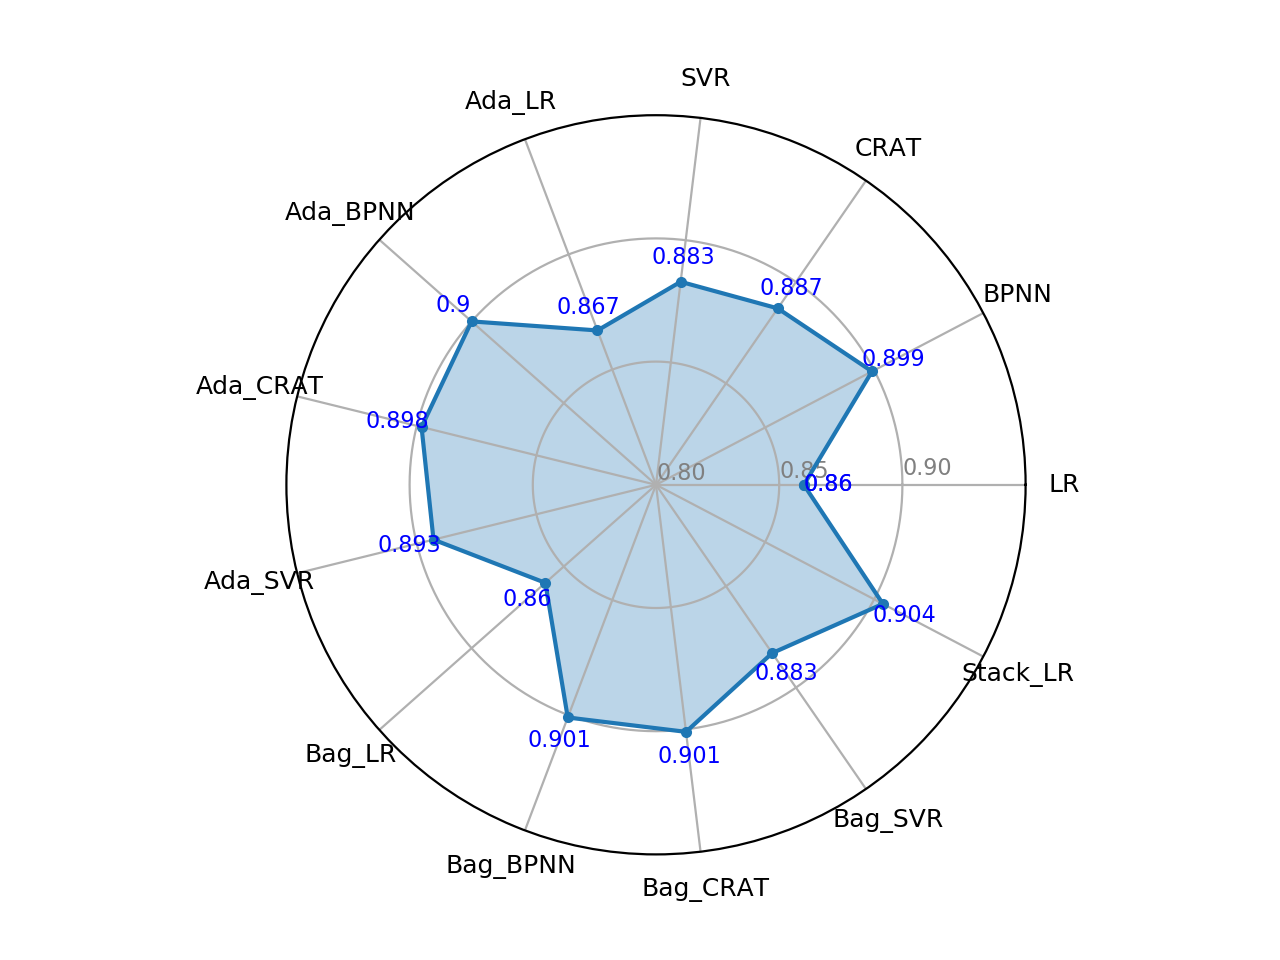
\includegraphics[width = \linewidth]{R2circle.png}
			\caption{$R^2$}
		\end{subfigure}%
		\hspace{1em}
%		\subfigure[MAE ]{%
%			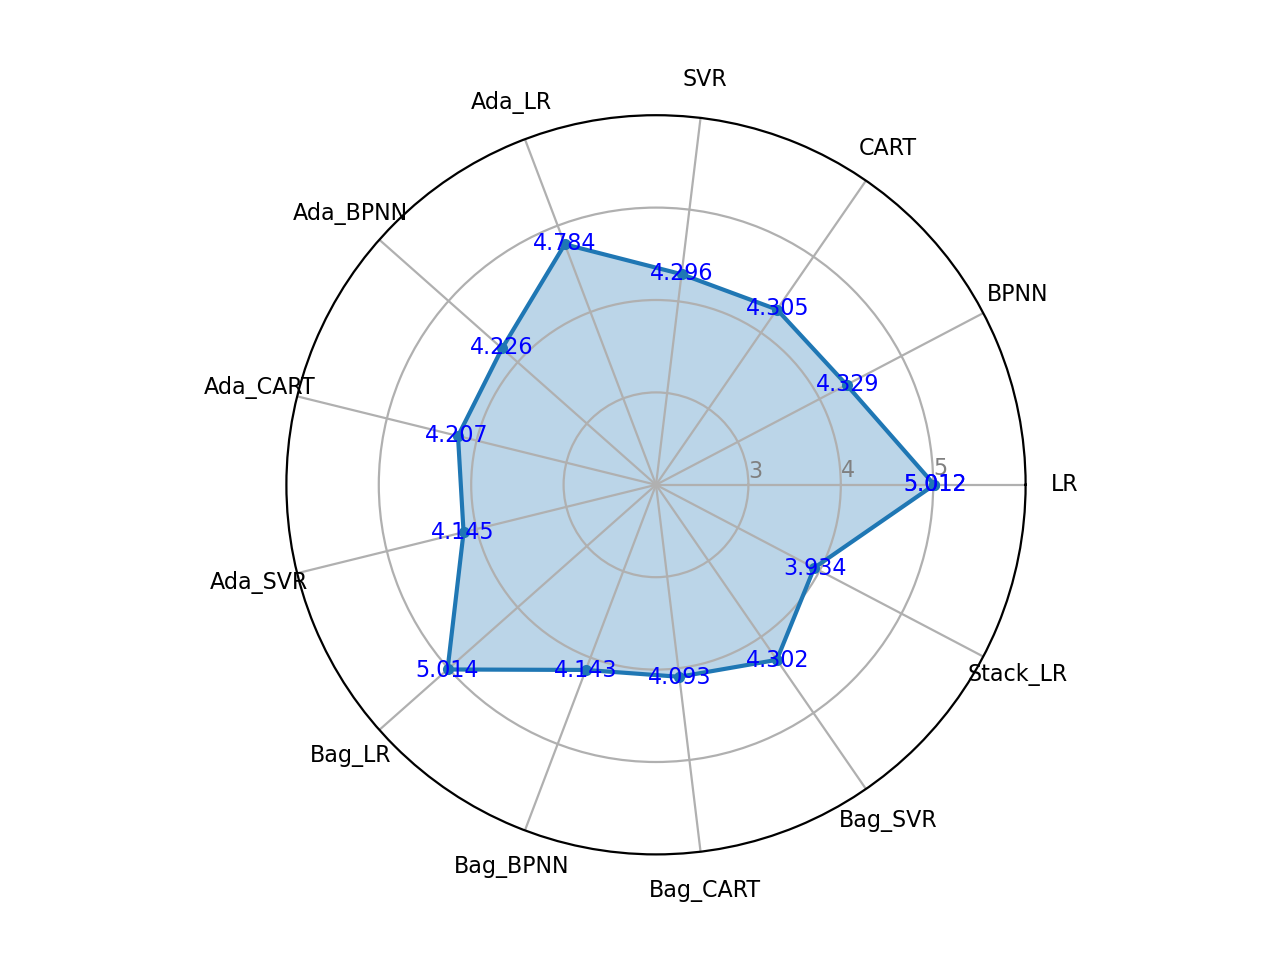
\includegraphics[width=.6\textwidth]{MAEcircle.png}}\hspace*{-1em} \hfill
%		\subfigure[RMSE]{%
%			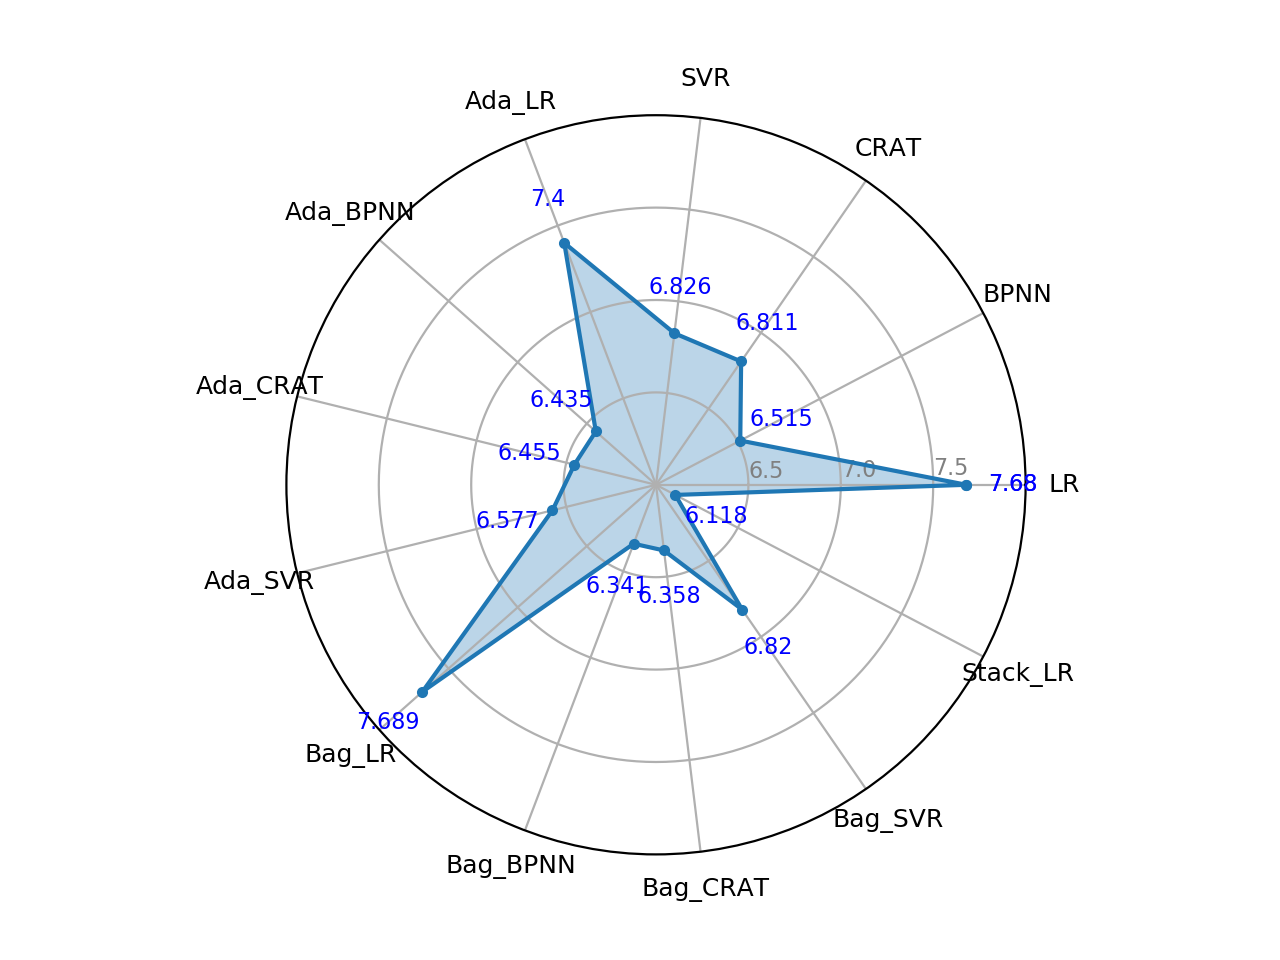
\includegraphics[width=.6\textwidth]{RMSEcircle.png}} \hfill
%		\subfigure[$R^2$]{%
%			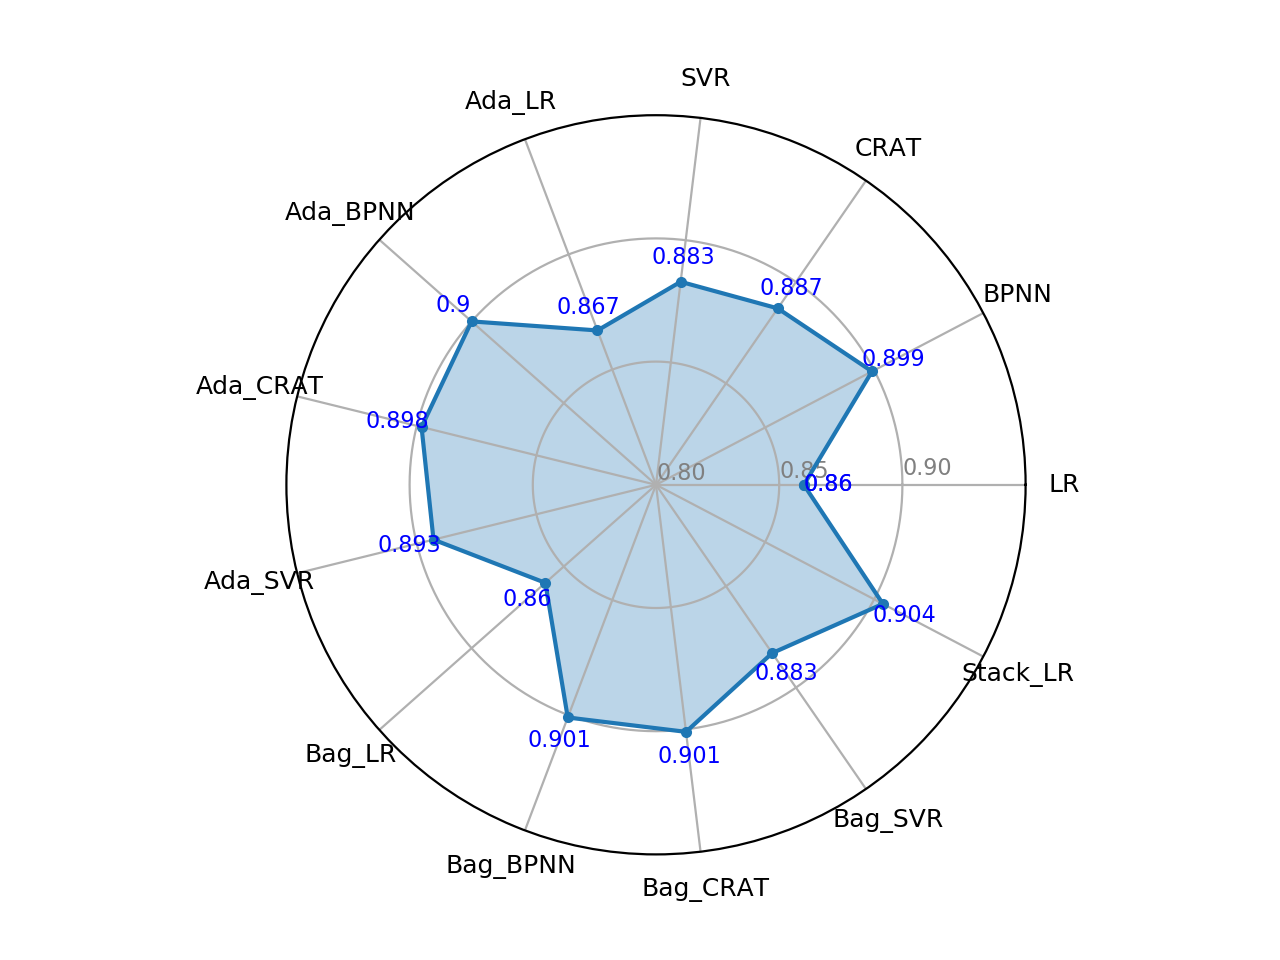
\includegraphics[width=.6\textwidth]{R2circle.png}}\hfill
		\caption{Average prediction performance of 10-fold cross-validation on all machine learning models for predicting self-healing ability of ECC }\label{comp}
	\end{figure}
	









	Overall, all models can noticeably reduce the error values and increase the prediction accuracy compared with LR, except Bag\_LR. For example, of the models based on ensemble learning by AdaBoost, Ada\_SVR performs the best on MAE, reducing by 17.3\%, Ada\_BPNN performs the best on RMSE, reducing by 16.2\% and on $R^2$, increasing by 4.7\%. For the bagging ensemble methods, Bag\_CRAT performs the best on MAE, reducing by 18.3\%, Bag\_BPNN performs the best on RMSE, reducing by 17.4\%, and Bag\_CRAT and Bag\_BPNN have the same performance on $R^2$, increasing by 4.8\%. However, note that Bag\_LR has a worse performance than LR in terms of MAE and RMSE. This may result from several training examples repeatedly appearing in different replicated datasets to train multiple base regressors. 


	Table \ref{com} further shows the deviation of ensemble models from individual models which are used as base learners over the three statistical measures based on ten-fold cross-validation results. The results indicate that the ensemble methods using individual methods as a learning base improved the performance of the individual method on the basis of all three performance measures. For example, using BPNN as the learning base, ensemble method Bag\_BPNN has the lower error (MAE and RMSE decreasing by 4.3\% and 2.7\%, respectively) and higher accuracy ($R^2$ increasing by 0.2\%) than the individual method BPNN. Moreover, the comparative results showed that ensemble learning based models (Stack\_LR) distinctly outperformed the single learning based models (Ada\_LR and Bag\_LR) in terms of overall performance measures.
	
	\begin{table}[!h]
		\small
		\centering
		\caption{Performance deviation of ensemble models from benchmark models on self-healing of ECC }
		\begin{tabular*}{0.9\textwidth}{llccc|llccc}
			\toprule
			&	&	MAE	&	RMSE	&	$R^2$	&	&	&	MAE	&	RMSE	&	$R^2$	\\
			\cmidrule{3-5} \cmidrule{8-10}
			Benchmark & Model& \multicolumn{3}{c|}{$Dev (\%)$} &Benchmark & Model& \multicolumn{3}{c}{$Dev (\%)$} \\
			\midrule
			LR	&	Ada\_LR	&	-4.6	&	-3.6	&	0.8		&	LR	&	Bag\_LR	&	0.0	&	0.1	&	0.0	\\
			BPNN	&	Ada\_BPNN	&	-2.4	&	-1.2	&	0.1	&	BPNN	&	Bag\_BPNN	&	-4.3	&	-2.7	&	0.2	\\
			CRAT	&	Ada\_CRAT	&-2.3	&	-5.2	&	1.2	&	CRAT	&	Bag\_CRAT	&	-4.9	&	-6.6	&	1.6\\
			SVR	&	Ada\_SVR&-3.5	&	-3.6&	1.1	&	SVR	&	Bag\_SVR	&	0.1	&	-0.1	&	0.0	\\
			\midrule
			Ada\_LR	&	Stack\_LR	&	-17.8&	-17.3&	4.3	&	Bag\_LR	&	Stack\_LR	&-21.5	&	-20.4&	5.1 \\
			\bottomrule 
		\end{tabular*}
		\label{com}
	\end{table} 
	
	
	
	Specifically, bagging ensembles substantially enhance the performance of BPNN and CRAT while the AdaBoost ensemble achieve a considerable improvement for LR and SVR. It means that BPNN and CRAT used as the base learner, bagging method achieves better results (lower error value and higher $R^2$) than the AdaBoost and individual method, and the LR and SVR used as the base learner, the AdaBoost method gets better results than the bagging and individual method.
	
	\subsection{Comparison of predicted and observed crack width}
	
	The comparison of the proposed ML models for the prediction outputs is illustrated in Figure \ref{error1} to \ref{error4}, in which the predicted crack width after self-healing by ML models and the experimental observed crack width after self-healing are first presented in sub -figure (a). In the rest of sub-figures, the error of predicted crack width over experimental observed crack width after self-healing is displayed as the measurement index based on the group of crack width before self-healing. Mostly, the smaller crack width before self-healing 
	%先给参考文献,说明,裂缝越小越容易修复,从图中可以,越小的裂缝
%	初始crack宽度越小,那么crack更倾向于被完全修复,那么crack width after self-healing就为零,那么预测值与实际值的差异就越小。
	
	
	
	Furthermore, a horizontal line located at the vertical coordinate of zero was taken as the target line in the rest of sub-figures. Generally, the error bar is shorter (indicates a closer distance from the target line) demonstrates the predicted crack width is more accurate. 
	
	It is can be seen from the Figure \ref{error1} that individual models, BPNN, CRAT and SVR 	
	
	\begin{figure}[!h]
		\centering
		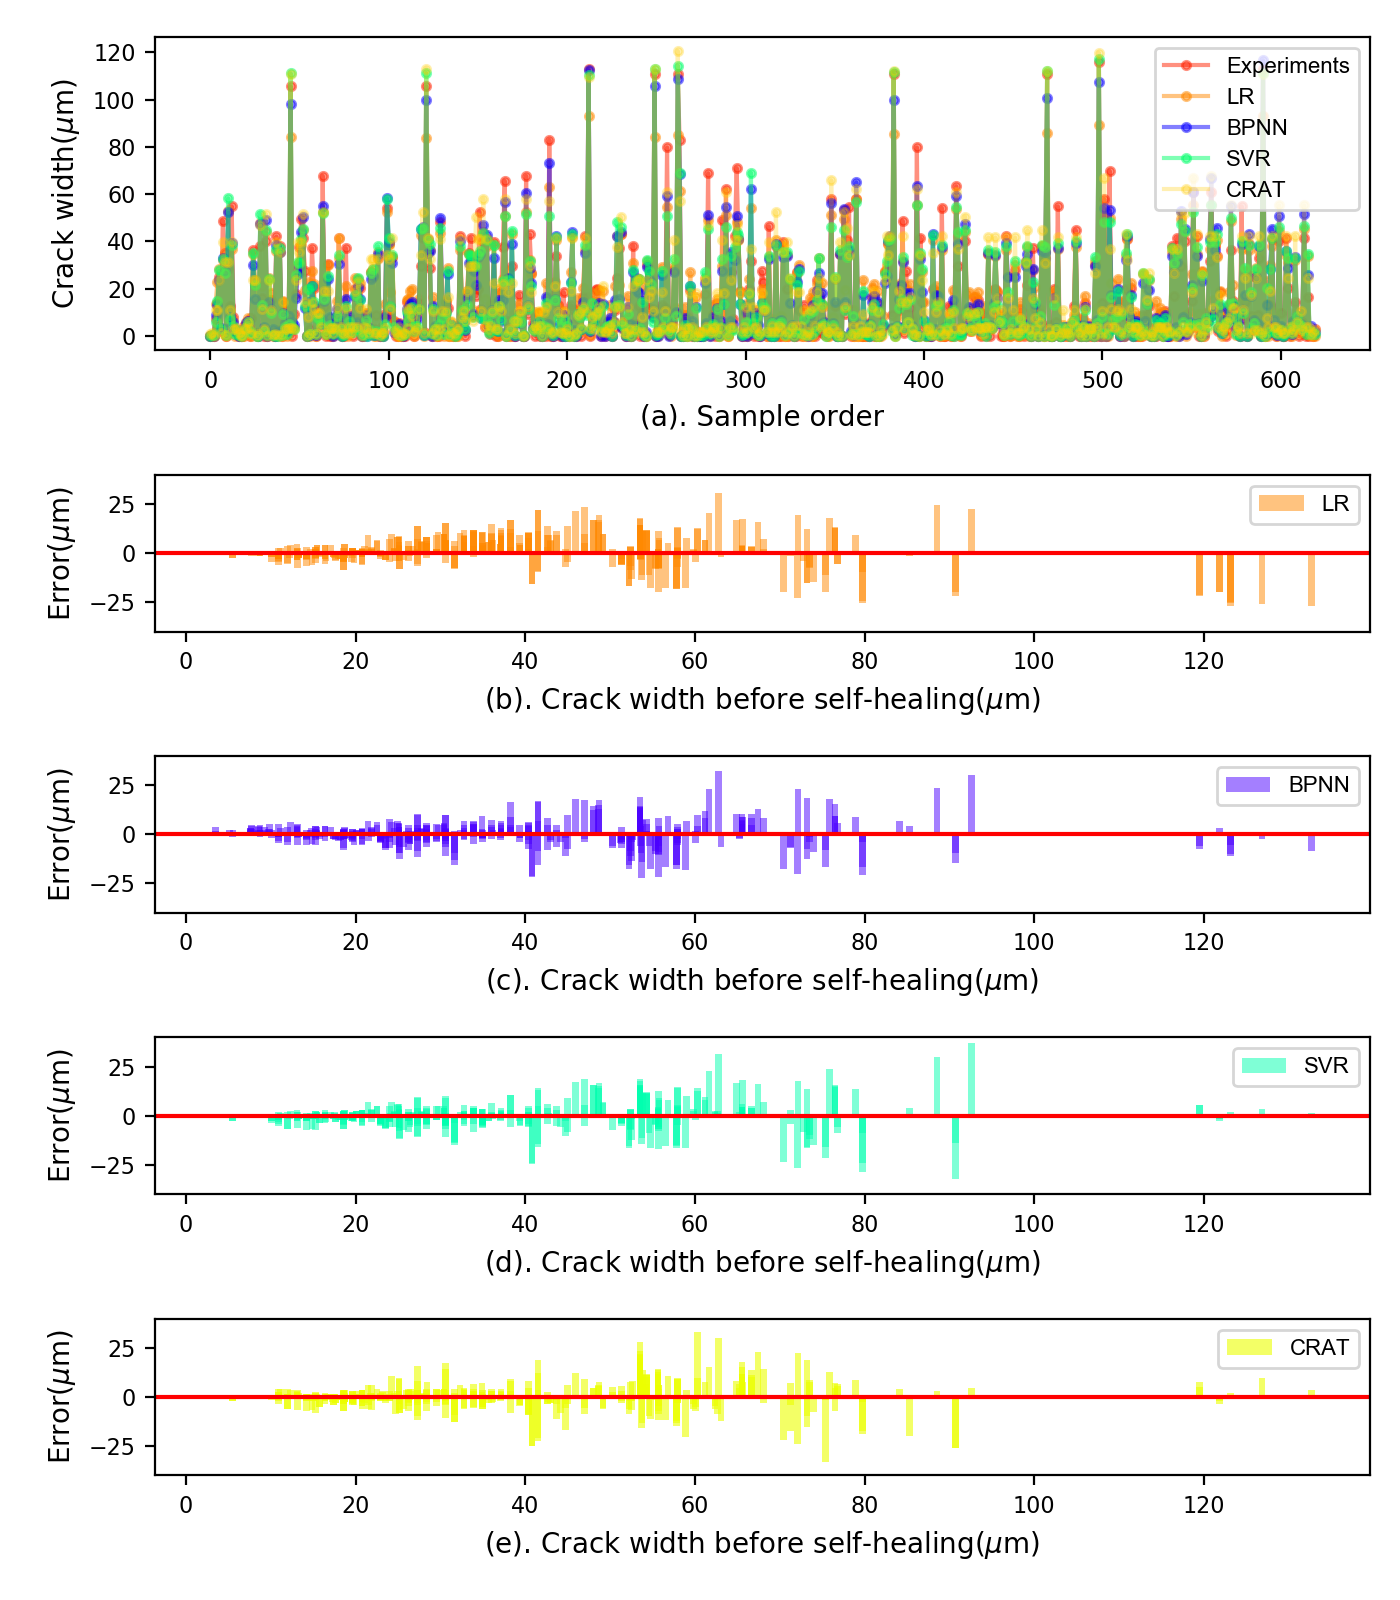
\includegraphics[width=\textwidth]{error.png}
		\caption{Comparison of predicted and observed crack width after self-healing of ECC for individual models}
		\label{error1}
	\end{figure}
	
			\begin{figure}[!h]
		\centering
		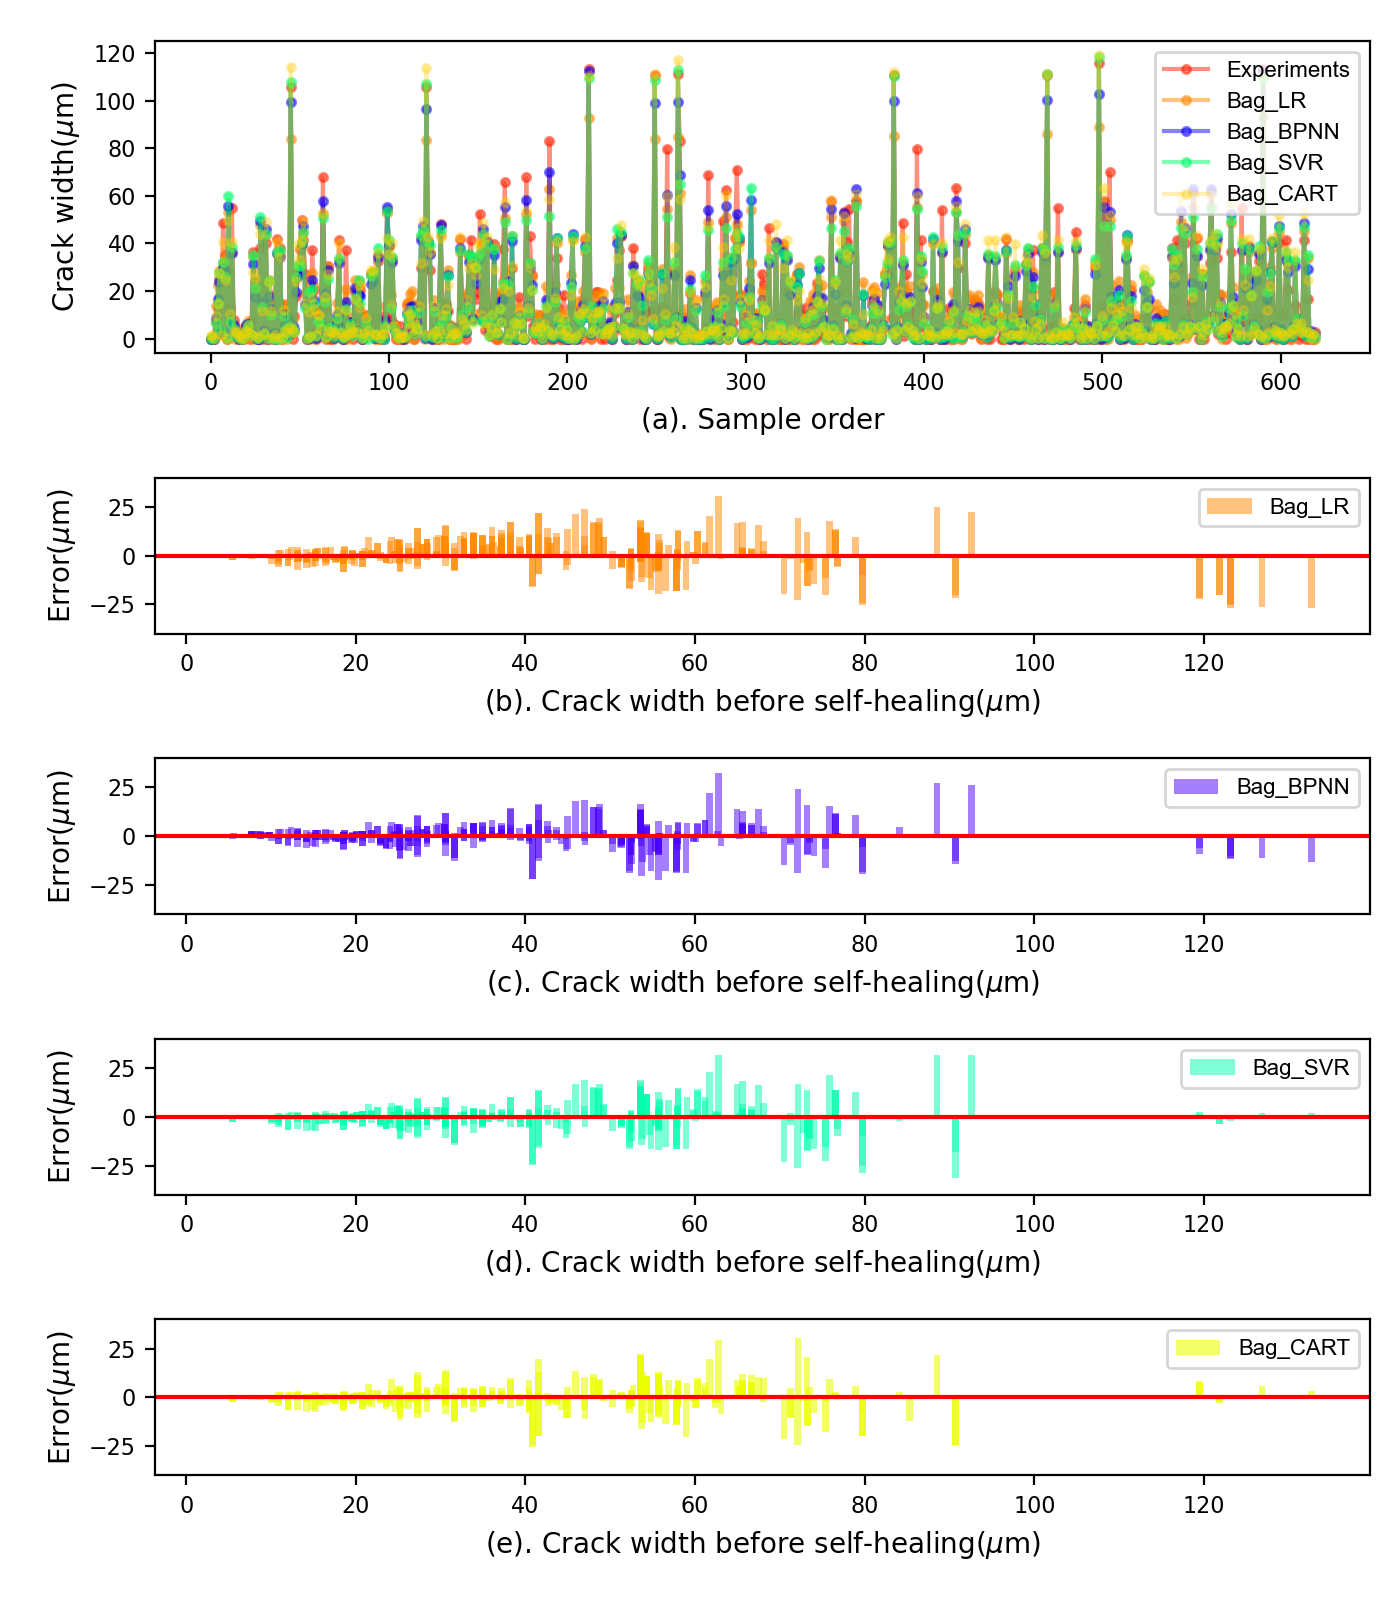
\includegraphics[width=\textwidth]{bagError.png}
		\caption{Comparison of predicted and observed crack width after self-healing of ECC for  bagging ensemble models}
		\label{error2}
	\end{figure}
	
		\begin{figure}[!h]
		\centering
		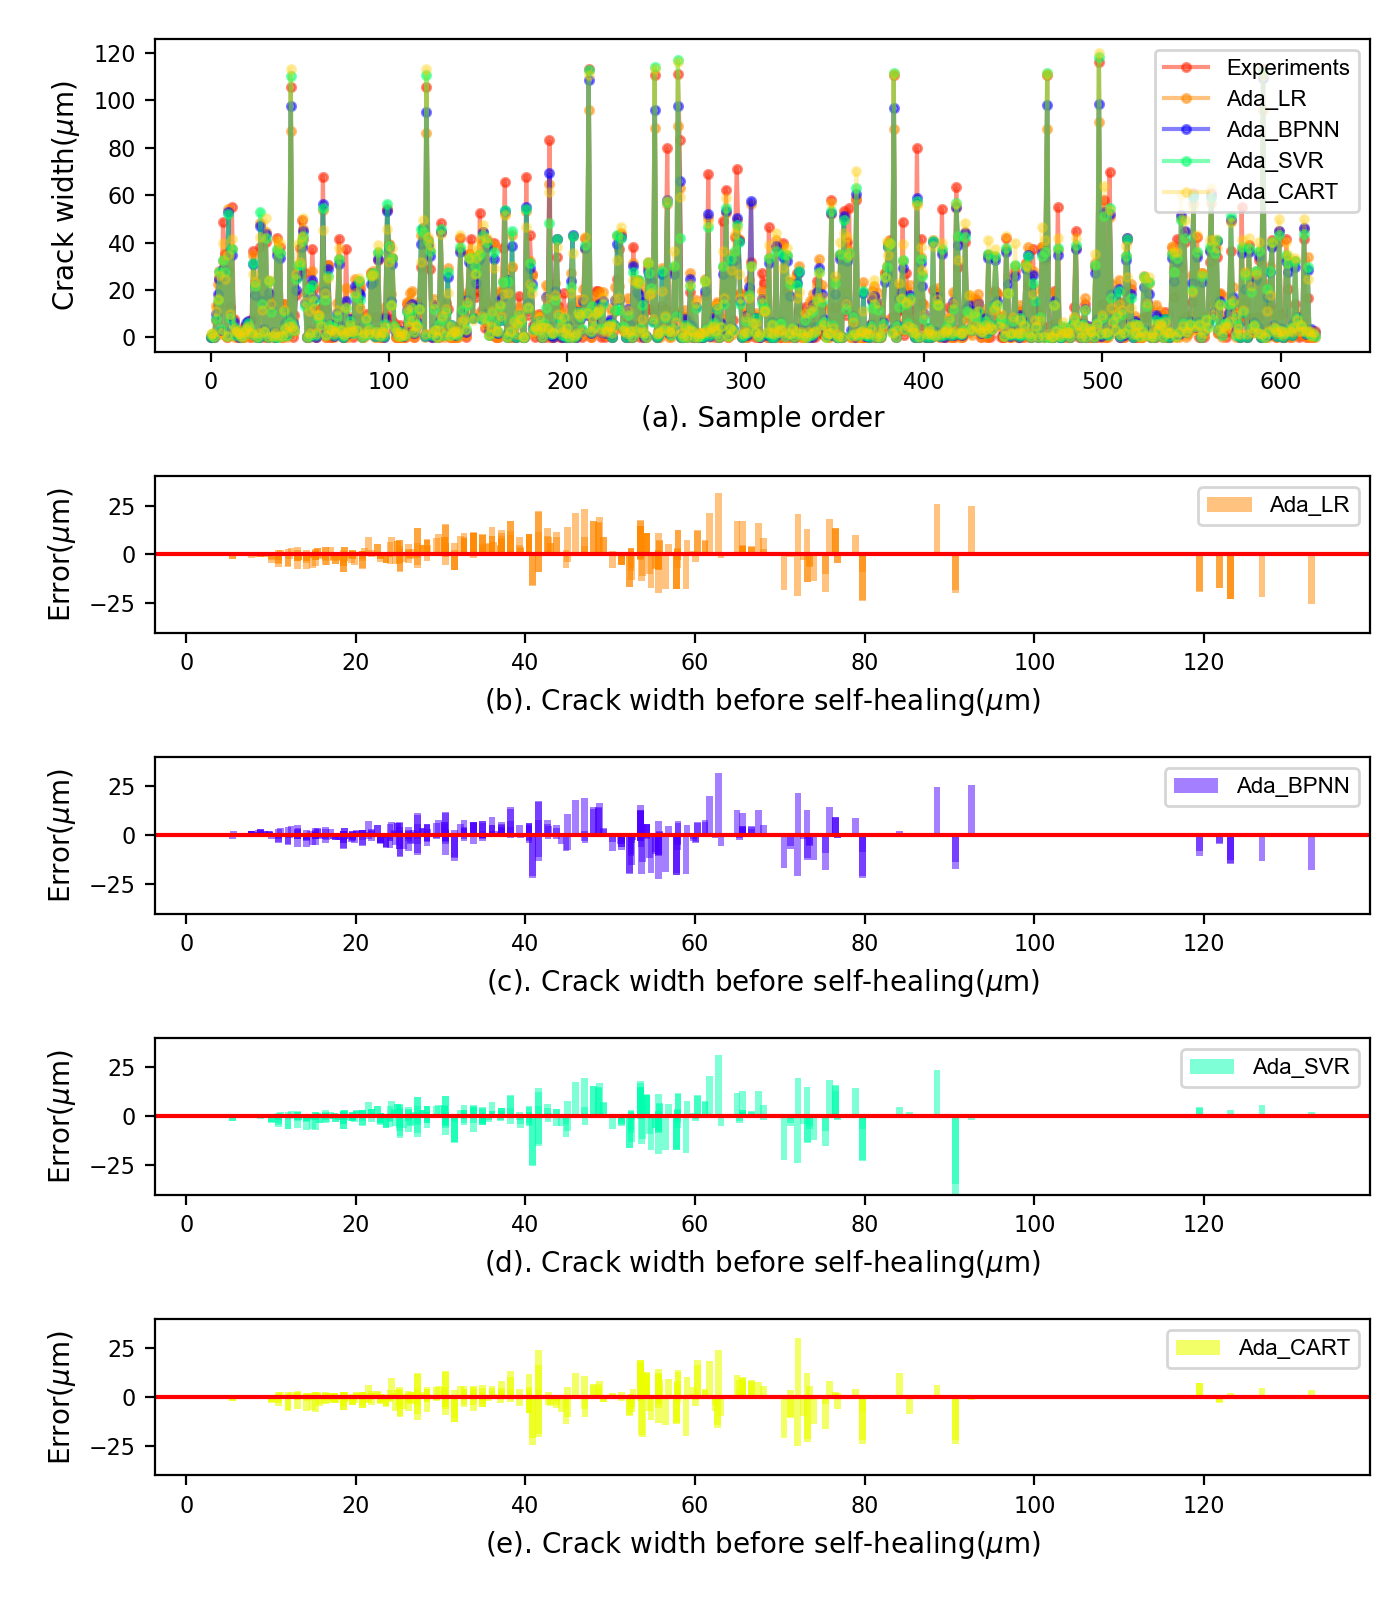
\includegraphics[width=\textwidth]{AdaError.png}
		\caption{Comparison of predicted and observed crack width after self-healing of ECC for  adaBoost ensemble models}
		\label{error3}
	\end{figure}

		\begin{figure}[!h]
	\centering
	\includegraphics[width=\textwidth]{StackError.png}
	\caption{Comparison of predicted and observed crack width after self-healing of ECC for  stacking ensemble models}
	\label{error4}
\end{figure}
	
	

	
	
	\begin{figure}[!h]
		\centering
		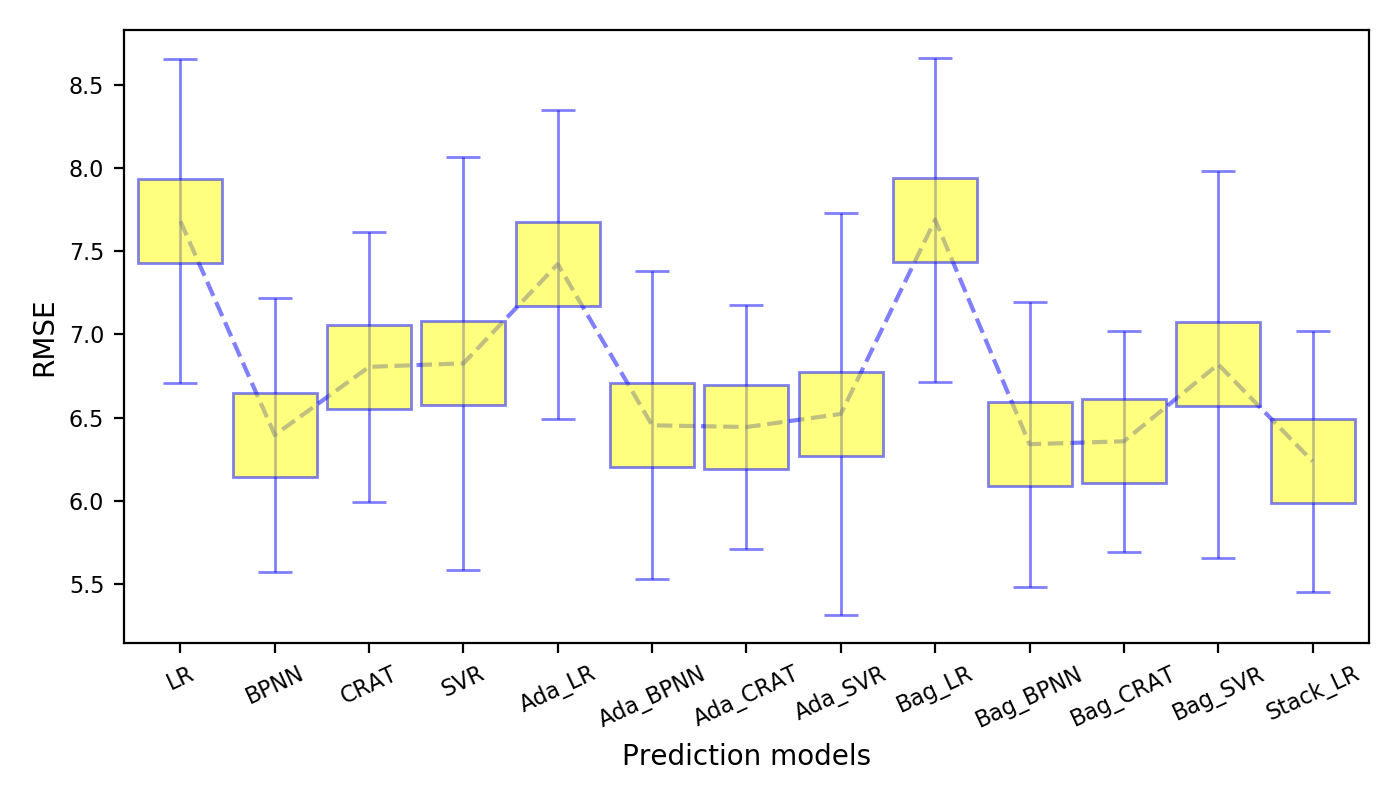
\includegraphics[width=\textwidth]{rmseBar.png}
		\caption{Comparison of predicted and observed crack width after self-healing of ECC for  stacking ensemble models}
		\label{bar}
	\end{figure}
	
	
	
The comparison of observed and predicted crack width after self-healing of ECC as the self-healing capability of ECC by all machine learning techniques is presented in Figures \ref{gbrt}. For example, plot \textit{(a)} presents the predicted crack width after self-healing of ECC by LR model, which has $R^2$ coefficient for 0.860 and the slope of the straight line for 0.799. As it can be seen, the Stack\_LR has the best performance and obtained a better fit to a straight line with the slope of 0.899 and $R^2$ coefficient of 0.904. In Stack\_LR, the predicted value of crack width after self-healing of ECC adheres to the line ($Y=X$) better than other models, which indicates more accuracy for predicting self-healing of ECC. In addition, Figures \ref{gbrt} reveal the empirical data of crack width after self-healing of ECC generated from laboratory experiments is mainly distributed between $0$ to $80 \mu m$. Whereas a few samples have a crack width over $100 \mu m$.  This insufficient data may result in machine learning models being trained inadequately and reducing the prediction accuracy.  

	The comparative analysis of observed and predicted crack width after self-healing of ECC as the self-healing capability of ECC by all machine learning techniques is presented in Figures \ref{f4:lr} to \ref{f4:stack}. The coefficient of determination $R^2$ and equation of the linear least square fit line are shown in these Figures (of the form $y = ax +b$ relating predicted crack width $``y"$ after self-healing which is the dependent variable to experimental observed crack width $``x"$ after self-healing which is an independent variable) indicates that the prediction output is very close to the experimental observed results. Basically, the more closely the $R^2$ approaches to one, and with the slope $``a"$ of the fit line is closer to 1 and the $``y"$ intercept $``b"$ is more small, close to 0 (the fit line is more close to the target line $Y = X$), the better the prediction performance is achieved. It can be seen from Figure \ref{f4:lr}, for the LR model, the predicted crack width after self-healing has a reasonable performance with the coefficient $R^2$ for 0.860, and the slope $``a"$ of the fit line for 0.799 and the $``y"$ intercept $``b"$ is 3.804. Similarly, as it can be seen in Figure \ref{f4:lb}, the BPNN model has a better performance than the LR model, which has the coefficient $R^2$ for 0.899, and the slope $``a"$ of the fit line for 0.866 and the $``y"$ intercept $``b"$ is 1.817. And as shown in Figure \ref{f4:lr} and \ref{f4:lb}, the predicted value of crack width after self-healing of ECC in the BPNN model adheres to the target line $Y = X$ better than the LR model, especially for the crack width over 100 $\mu m$, which further indicates the BPNN model is more accuracy and outperform the LR model.  Specifically, the Stack\_LR model has the best performance with the coefficient $R^2$ for 0.904, and has the slope $``a"$ of the fit line for 0.899 (close to 1) and the $``y"$ intercept $``b"$ is 1.579 (close to 0) as shown in Figure \ref{f4:stack}. In addition, Figures \ref{f4:lr} to \ref{f4:stack} reveal the experimental data of crack width after self-healing of ECC generated from laboratory experiments is mainly distributed between $0$ to $60 \mu m$. Whereas a few samples have a crack width over $100 \mu m$.  This insufficient data may result in machine learning models being trained inadequately and reducing the prediction accuracy.  
	
	
%	\begin{figure}[!h]
%		\centering
%		\subfigure[Comparison of observed ECC crack width and predicted ECC crack width after self-healing by LR ]{%
%			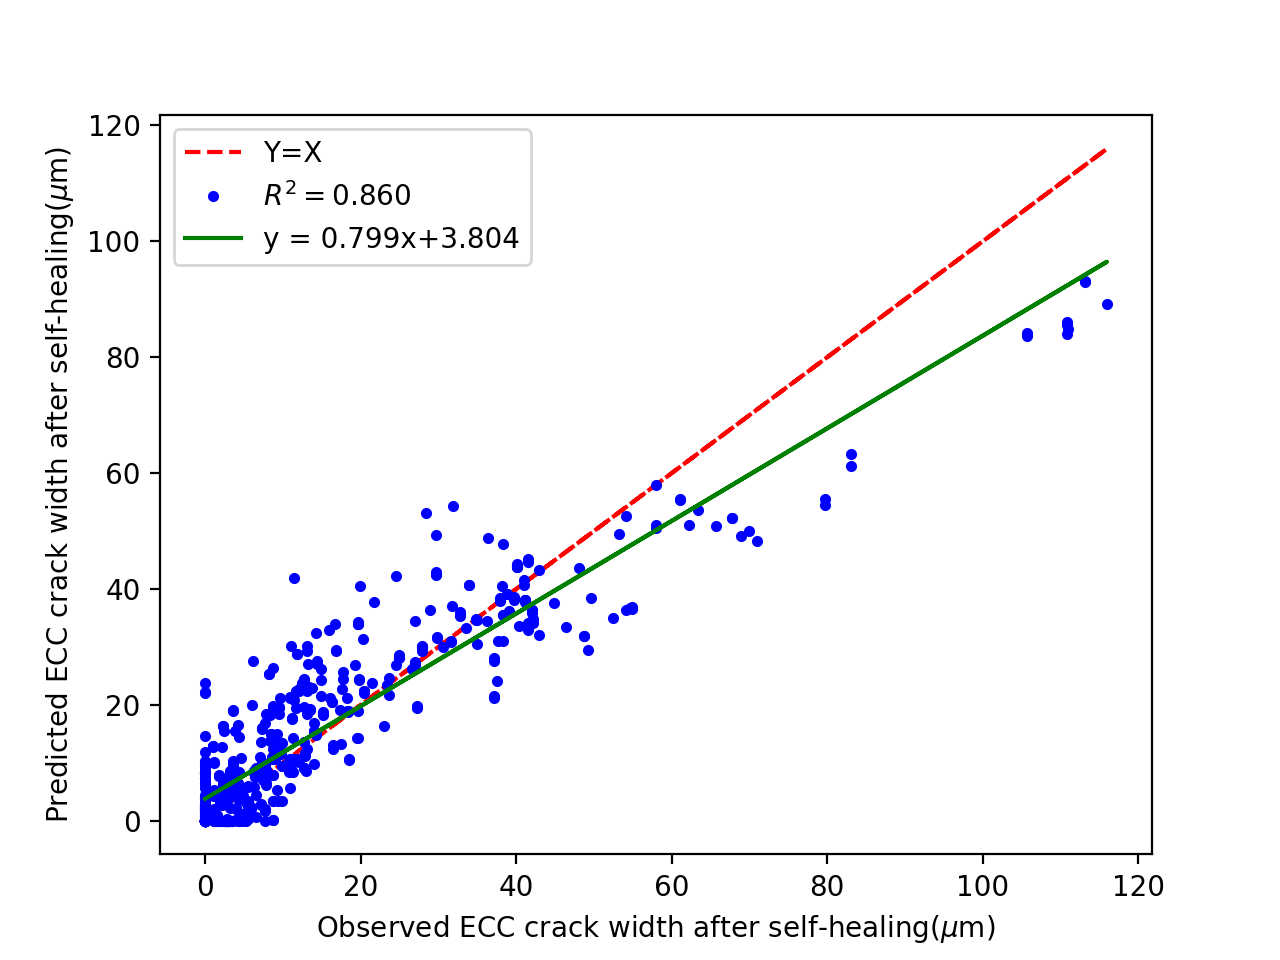
\includegraphics[width=.5\textwidth]{02LR.png}}\hfill
%		\subfigure[Comparison of observed ECC crack width and predicted ECC crack width after self-healing by BPNN ]{%
%			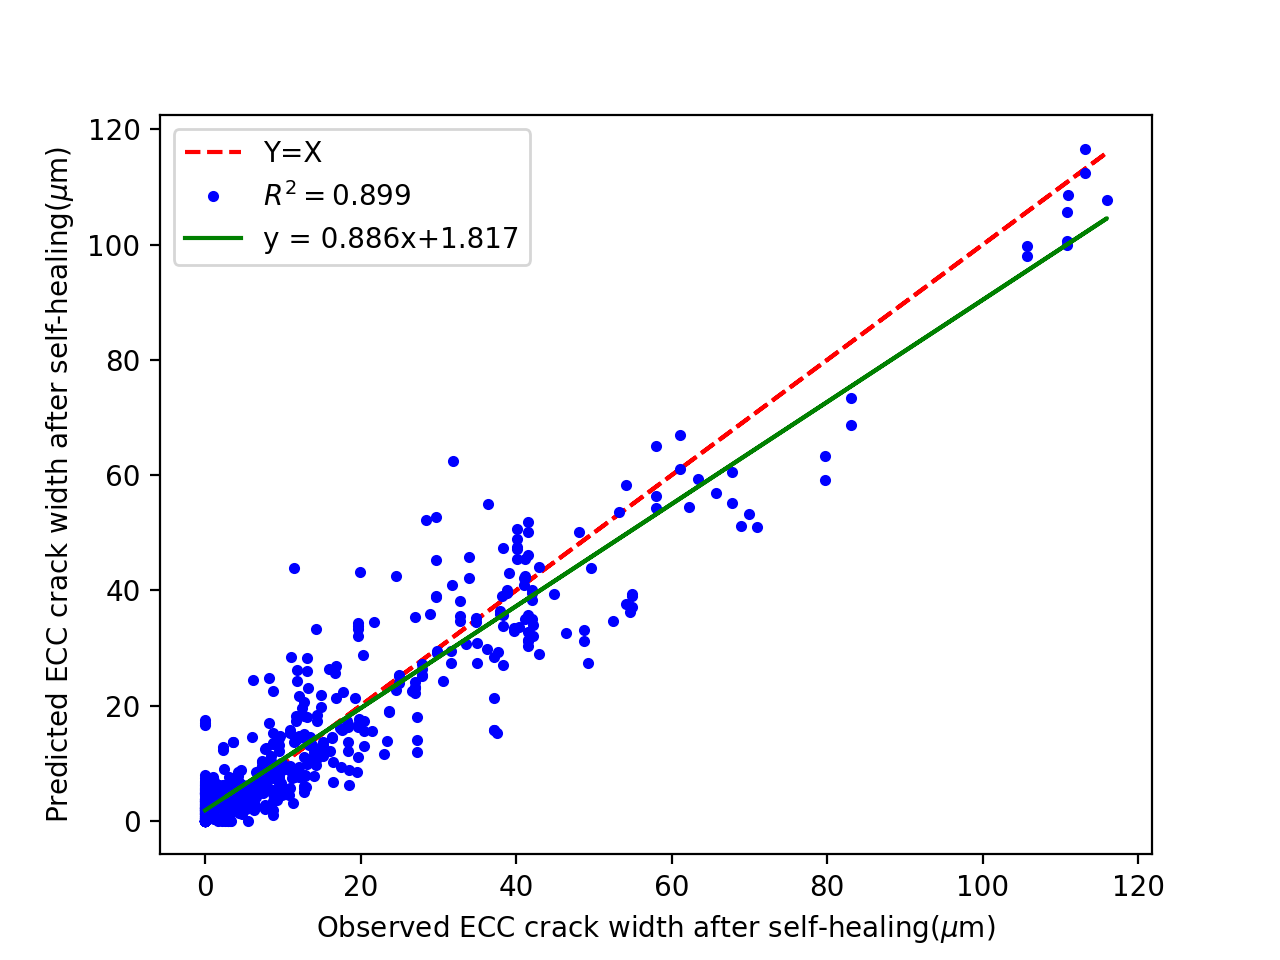
\includegraphics[width=.5\textwidth]{02BPNN.png}}\hfill
%		\subfigure[Comparison of observed ECC crack width and predicted ECC crack width after self-healing by Ada\_BPNN]{%
%			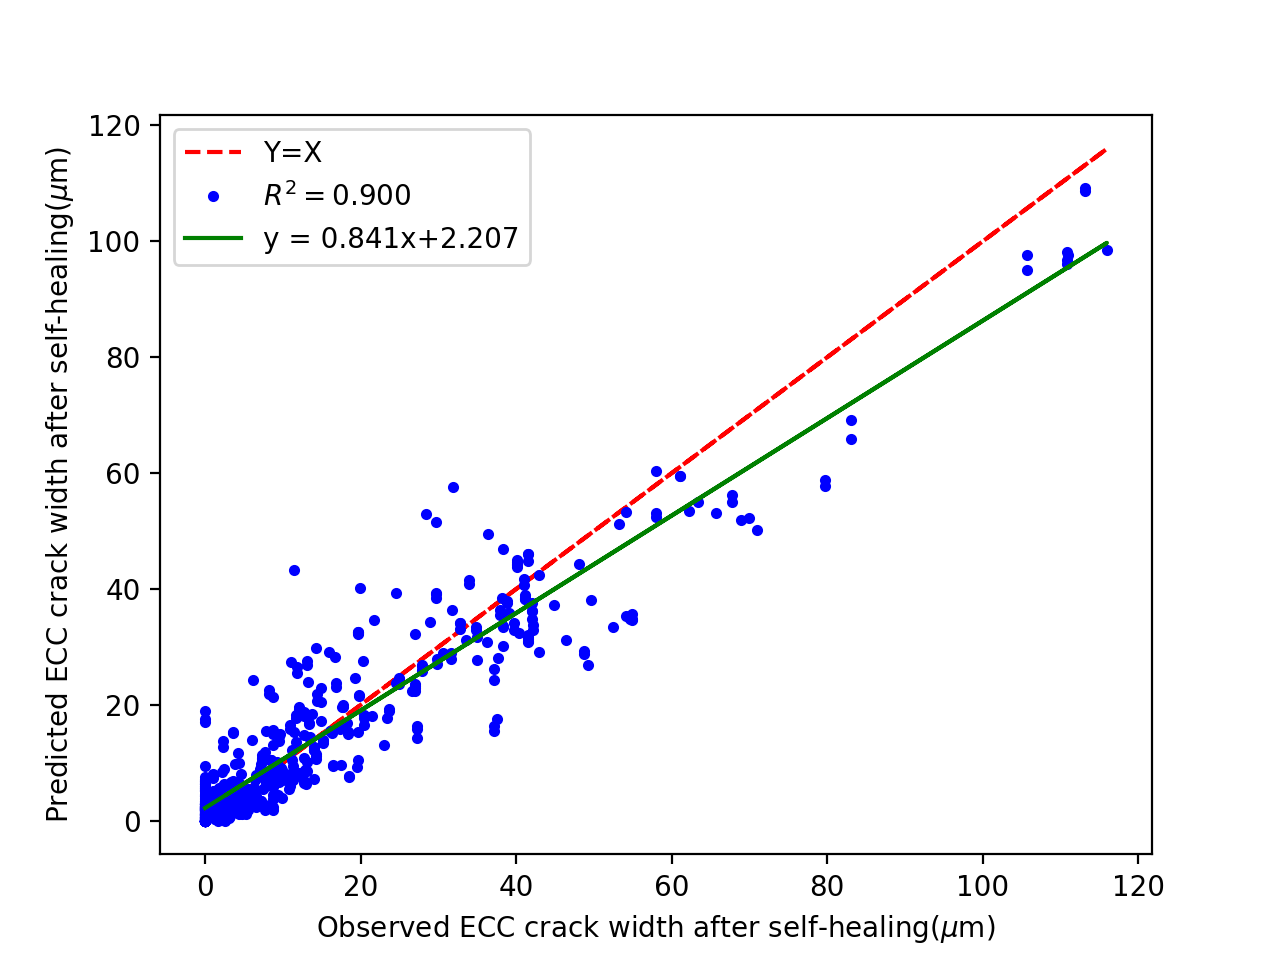
\includegraphics[width=.5\textwidth]{02Ada_BPNN.png}}\hfill
%		\subfigure[Comparison of observed ECC crack width and predicted ECC crack width after self-healing by Bag\_BPNN]{%
%			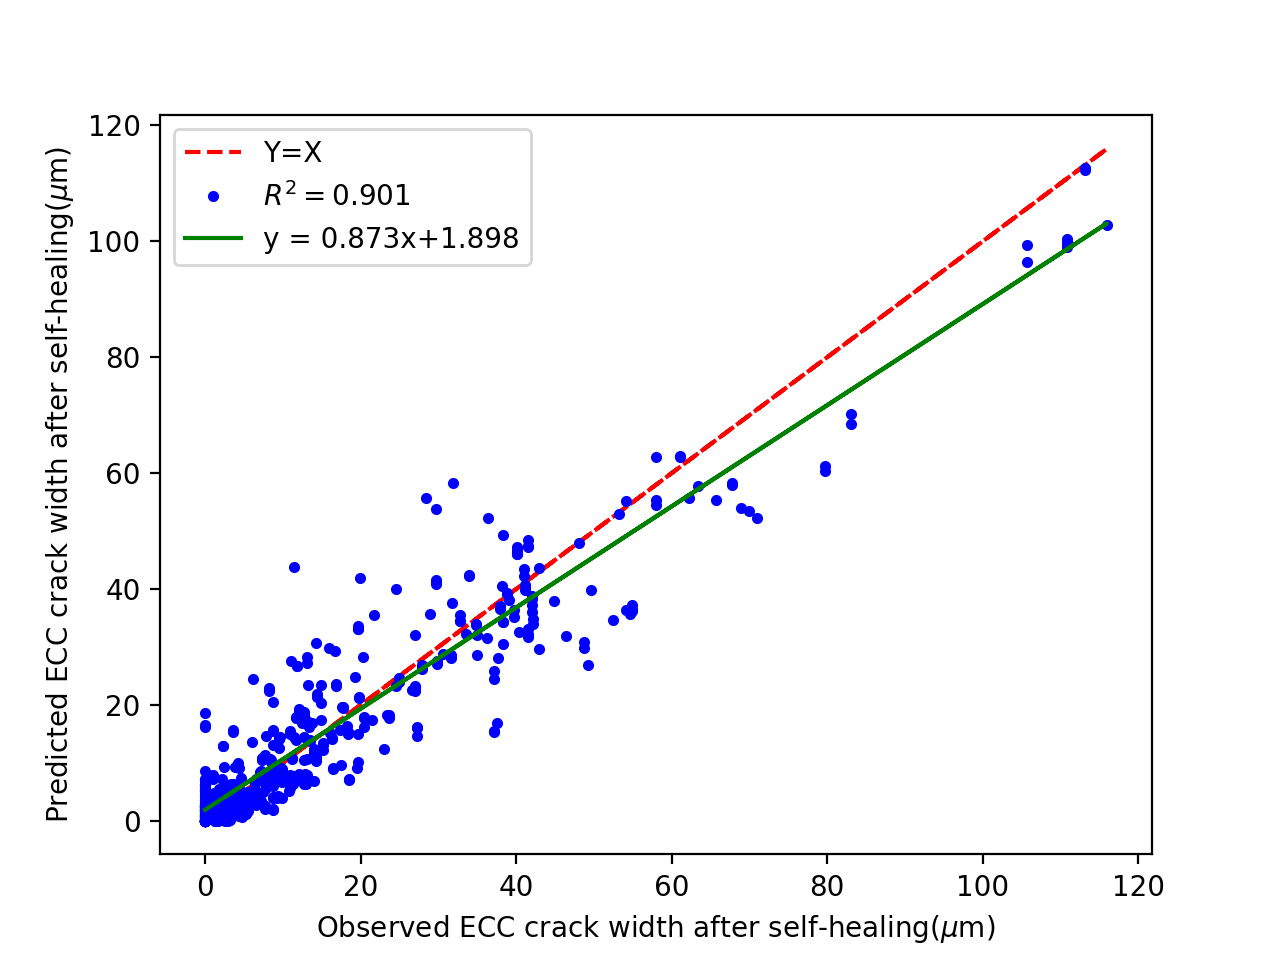
\includegraphics[width=.5\textwidth]{02Bag_BPNN.png}}\hfill
%		\subfigure[Comparison of observed ECC crack width and predicted ECC crack width after self-healing by Stack\_LR ]{%
%			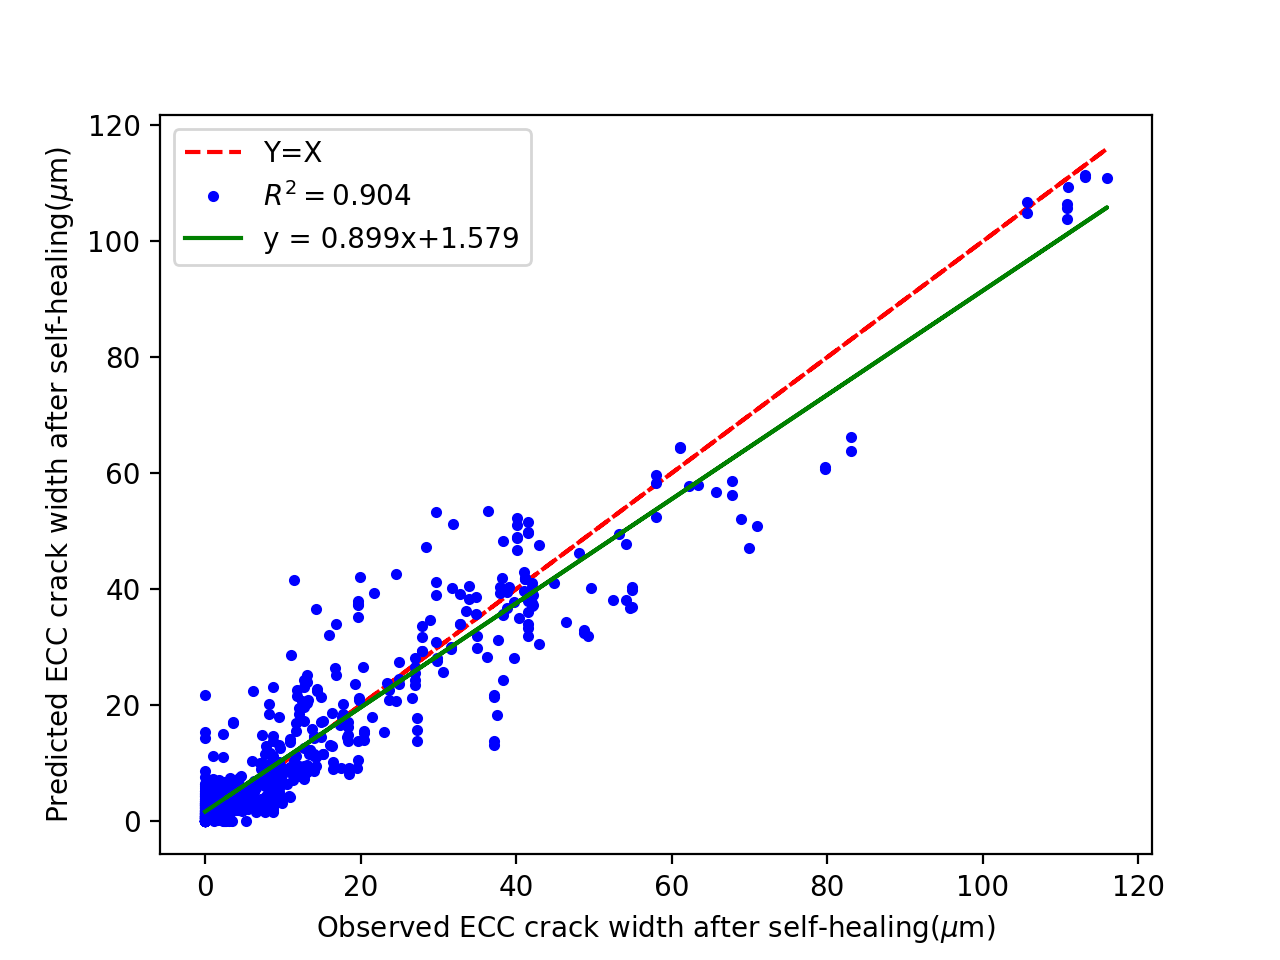
\includegraphics[width=.5\textwidth]{02Stack_LR.png}}\hfill
%		\caption{Comparison of observed ECC crack width and predicted ECC crack width after self-healing by individual and ensemble methods }\label{gbrt}
%	\end{figure}
	
	%%%%%%%%%%%%%%%%%%%%%%%%%%%%%%%%%%%%%%%%%%
	\section{Conclusions}
	\label{con}
	
	In this chapter, a comprehensive comparison is proposed to analyse the performance of prediction of the self-healing ability of ECC using individual and ensemble methods. All machine learning models are trained and tested based on the experimental results from nine ECC mixtures. The comparison results provide valuable insights into proposing and validating the machine learning models for predicting self-healing on ECC.
	
	A total of four individual methods (LR, BPNN, CRAT, and SVR) and three ensemble methods (bagging, AdaBoost, and stacking) are used to perform the prediction of the self-healing ability of ECC. In these, the performance of LR is used as a benchmark baseline to compare the performance of other individual and ensemble models.  The proposed ensemble methods, bagging and AdaBoost, use one of the four individual methods as a base estimator to aggregate multiple single learning based prediction. The stacking method is used to combine multiple predictions generated by multiple regression models (SVR, BPNN, and CRAT).  
	
	The Stack\_LR model demonstrated great predictive ability and the best performance among all individual and ensemble methods, showing the lowest error values on MAE 3.934 and RMSE 6.118 and the highest on $R^2$ 0.904. Moreover, all ensemble methods present the improvement of the predictive ability of individual methods. In particular, the bagging method obviously improves the prediction performance of CRAT on MAE 4.9\%, RMSE 6.6\%, and $R^2$ 1.6\%. On the other hand, the BPNN model performs the best in terms of RMSE and $R^2$ among all individual models.
	
	The computational results indicate the individual and ensemble methods can be used to predict the self-healing ability of ECC. However, how to choose a fit base learner for different ensemble methods is critical. Engineers engaged in the design of durable and sustainable ECC mixtures will benefit from the use of machine learning models. Also all individual and ensemble models can be used as a tool for the prediction of the properties of ECC and can be optimized to develop hybrid models for further improving predictive ability.
	
	Future investigation and experimentation will be considered to extend the training dataset to include various crack width distributions and diverse influencing factors, such as components, W/MC rate etc., on self-healing of ECC. And more research should be undertaken to explore how to optimize parameters in machine learning models and develop hybrid modelling strategies to improve the prediction accuracy.	
	
	
	
	%next line adds the Bibliography to the contents page
	\addcontentsline{toc}{chapter}{References}
	%uncomment next line to change bibliography name to references
	%\renewcommand{\bibname}{References}
	\bibliographystyle{unsrtnat}  %use the plain bibliography style
	\bibliography{refs}        %use a bibtex bibliography file refs.bib	
	
	
\end{document}